


        
        \section{Neutron stars in binary systems}
        \label{binary_NS}

            Astrophysical prospects for binary pulsar detection. 
            Binary pulsars are perhaps our best hope for detecting continuous gravitational waves.

%\begin{frame}{Neutron stars in binary systems}
\subsection{Continuous gravitational waves from neutron stars}

\begin{definition}
Neutron star with a partner in a binary system, 

e.g., a low-mass X-ray binary (LMXB)\end{definition}
\begin{example}
Scorpius X-1
\end{example}

Potential candidates for gravitational waves:
\begin{itemize}
\item Longer lifetime than isolated sources (recycling)
\item Ellipticity \& hot spots due to accretion
\item Torque balance hypothesis (Papaloizou \& Pringle 1978, Wagoner 1984):
\item \emph{bright ms pulsars}
\item Speed limit? (Chakrabarty 2003)
\end{itemize}
%\end{frame}




            \subsection{Binary spin-up and detectable lifetime}
            \label{spin-up}
         
                GW pulsar lifetime alone vs companion.

            \subsection{Detection rate projections}
            \label{rate_projections}

                aLIGO rate projections.

        \section{TwoSpect all-sky searches}
        \label{all-sky}

        General philosophy: LIGO continuous wave searches are matched filters, like inspiral searches. However, though the filter is easier (compared to the inspiral waveform) to calculate, the computational challenge is much harder (since we usually integrate over a longer timespan, compensating for weaker signals). Matched filtering a binary pulsar search in the time-domain, with complete phase information, would be computationally intractable in the early 2010s. However, by switching the problem to the frequency domain, and using power instead of amplitude, the search becomes feasible, albeit at a cost in sensitivity -- the detectable strain $h$ scales only as $T^{1/4}$ instead of $T^{1/2}$ for a coherent search.

            TwoSpect methods as-is. These are described in detail in Evan Goetz's thesis~\cite{GoetzThesis}. Note that the code is located on the web freely accessible in the LALApps repository~\cite{LALAPPSrepo}.

For primers on error analysis and statistics, see Taylor~\cite{taylor} as well as Casella and Berger~\cite{CasellaBerger2001}.

            \subsection{Two spectra: a double Fourier transform}
            \label{two_spectra}

                'Two spectra' -- FFT of periodograms reveals modulation of sine waves.

            \subsection{Infering neutron stars with companions}
            \label{inference}
 
                Infer whether modulation is due to a companion star.



%\begin{frame}{TwoSpect algorithm for all-sky binary searches}
\subsection{TwoSpect algorithm for all-sky binary searches}


\textbf{TwoSpect} (Goetz \& Riles 2011) searches for patterns in


doubly Fourier-transformed data from binary's orbital modulation


\emph{doubly Fourier-transformed:} $k$ frequency bins, time series
$n$


Short Fourier Transform series, along $n$, is FFT'd 


\[
R=\frac{\Sigma_{i=0}^{M-1}w(m_{i})[Z(m_{i})-\lambda(m_{i})]}{\Sigma_{i=0}^{M-1}[w(m_{i})]^{2}}
\]



$R$: template detection statistic


$w$: template weight


$i$: pixel index of $M$ pixels


$Z$: spectral power (after barycentric correction)


$\lambda$: expected noise power


$\rightarrow$ E. Goetz wrote, conducting all-sky search

%\end{frame}


% Everything below is imported from my APS and AEI talks (harmonized)

\begin{itemize}
\item Near term: direct binary searches toward promising targets
\item Long term: enhance all searches, start age of astronomy
\item TwoSpect binary searches -- directed, Sco X-1
\end{itemize}


\begin{figure}
\begin{center}
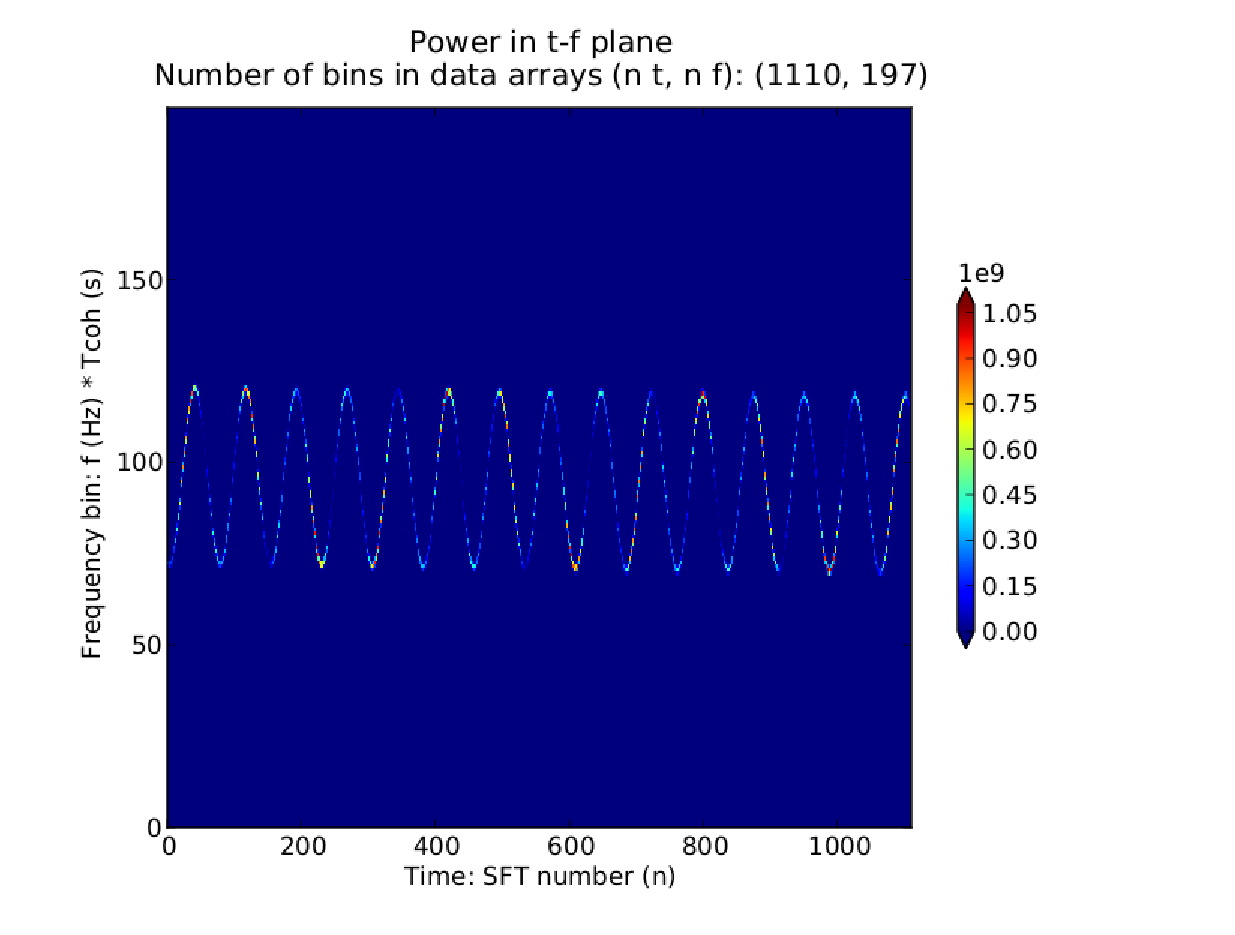
\includegraphics[width=0.8\paperwidth,height=0.4\paperheight]{tfplane-4e21-on-4e24.eps}
\caption{After Doppler-shifting the frequencies into the solar system barycenter, TwoSpect analyses begin on this first, time-frequency plane. A simulated signal at 100.015 Hz and $\textup{asini} = 1.44$ is injected with $h_0 = 4\times 10^{-21}$ into $10^6$ seconds of Gaussian noise at $Sh = 4 \times 10^{-24}$ (the projected minimum Advanced LIGO noise level); the signal period is 68023.8259 seconds, as with Scorpius X-1.}
\end{center}
\end{figure}

\begin{figure}
\begin{center}
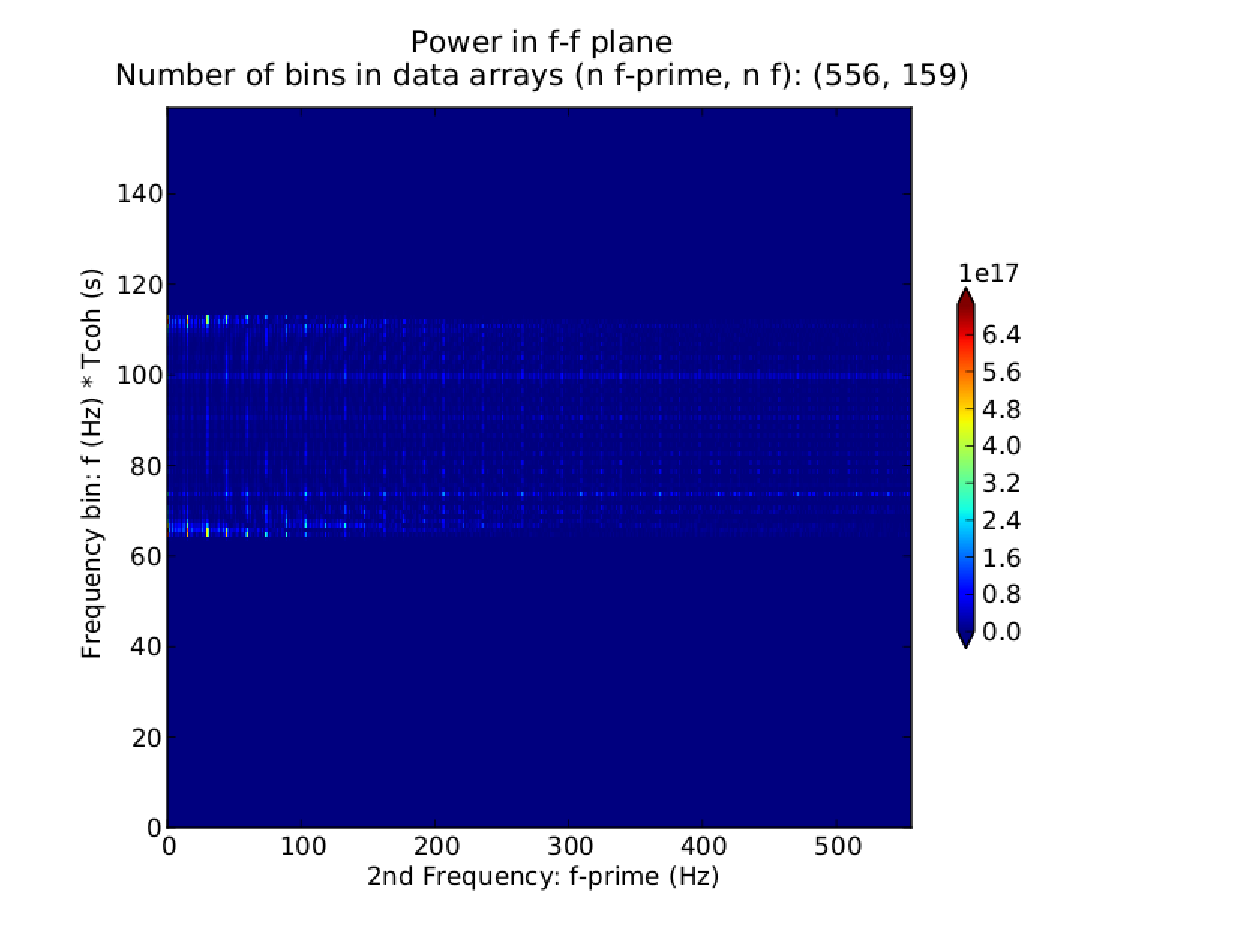
\includegraphics[width=0.8\paperwidth,height=0.4\paperheight]{ffplane-4e21-on-4e24.eps}
\caption{Fourier-transforming along the `rows' (constant frequency bin, variable time bin) generate a second plane, the frequency-frequency plane. The power of each bin in this transform is plotted as a pixel. By aggregating power, this second Fourier transform enhances signal so that matched templates can be applied for a search.}
\end{center}
\end{figure}

\begin{figure}
\begin{center}
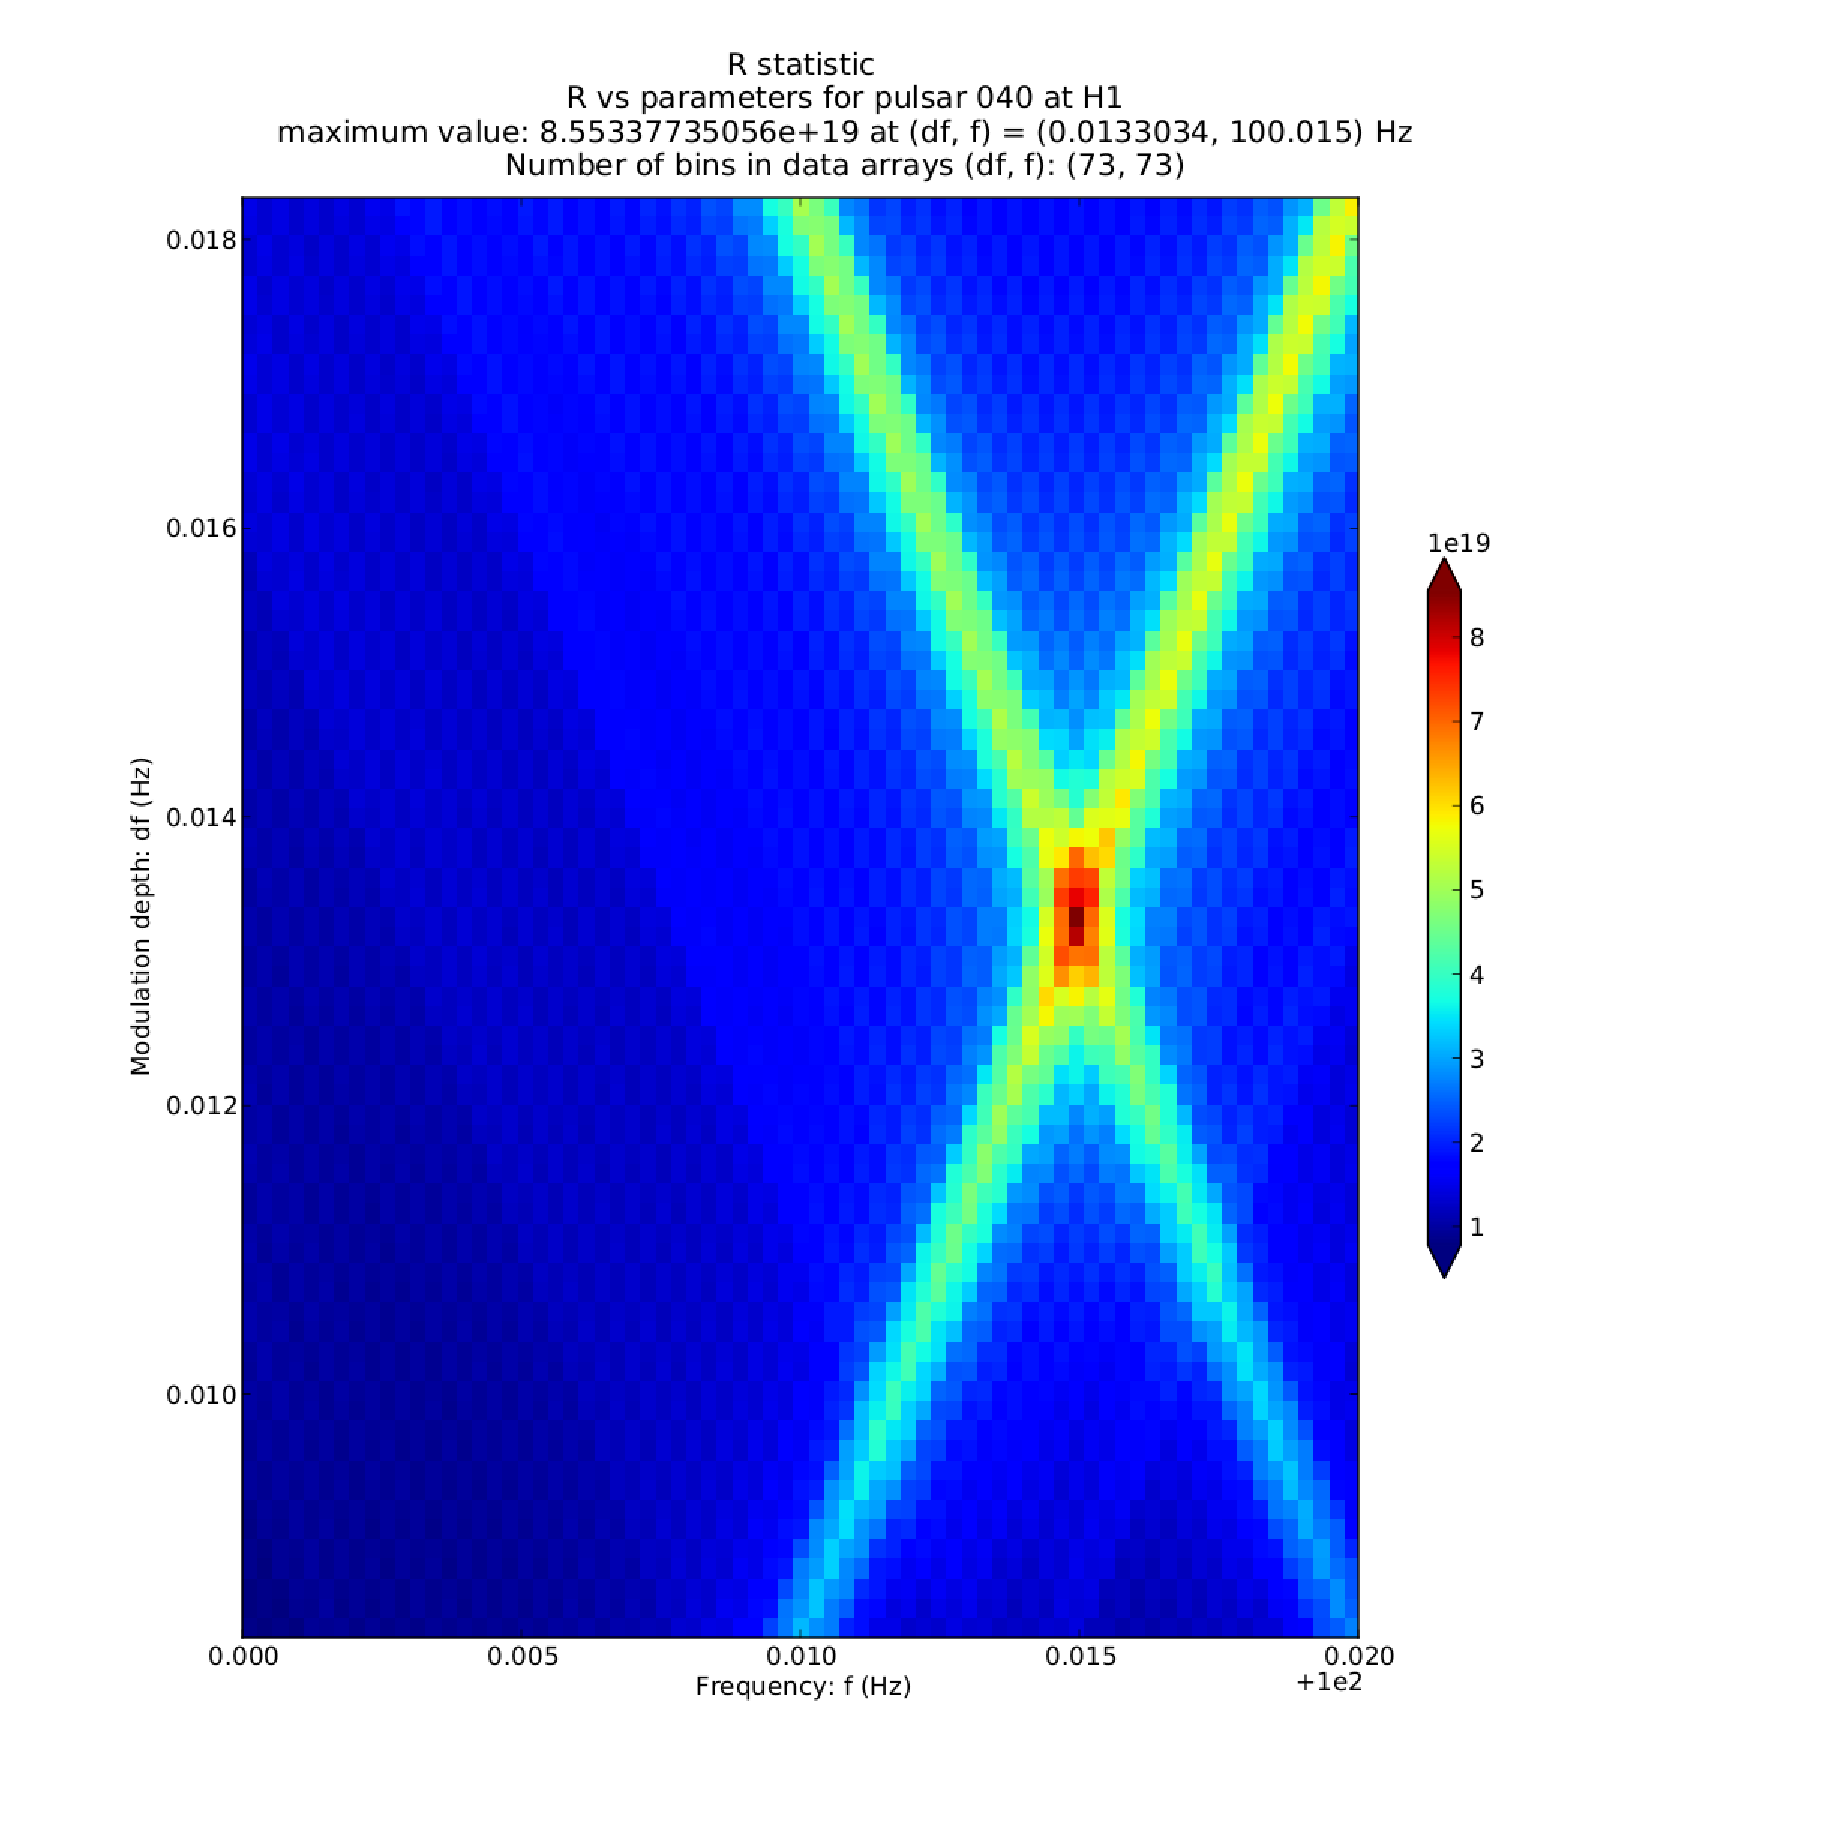
\includegraphics[width=0.8\paperwidth,height=0.62\paperheight]{R-4e21-on-4e24.eps}
\caption{Exact templates for putative singals weight the pixels in the frequency-frequency plane to generate $R$ statistic for a simulated pulsar (note: not the same as pulsar $40$ in the Scorpius X-1 mock data challenge) at 100.015 Hz and $\textup{asini} = 1.44$. The resulting $R$ values are heatmap-plotted on the modulation depth vs frequency plane.}
\end{center}
\end{figure}

\begin{figure}
\begin{center}
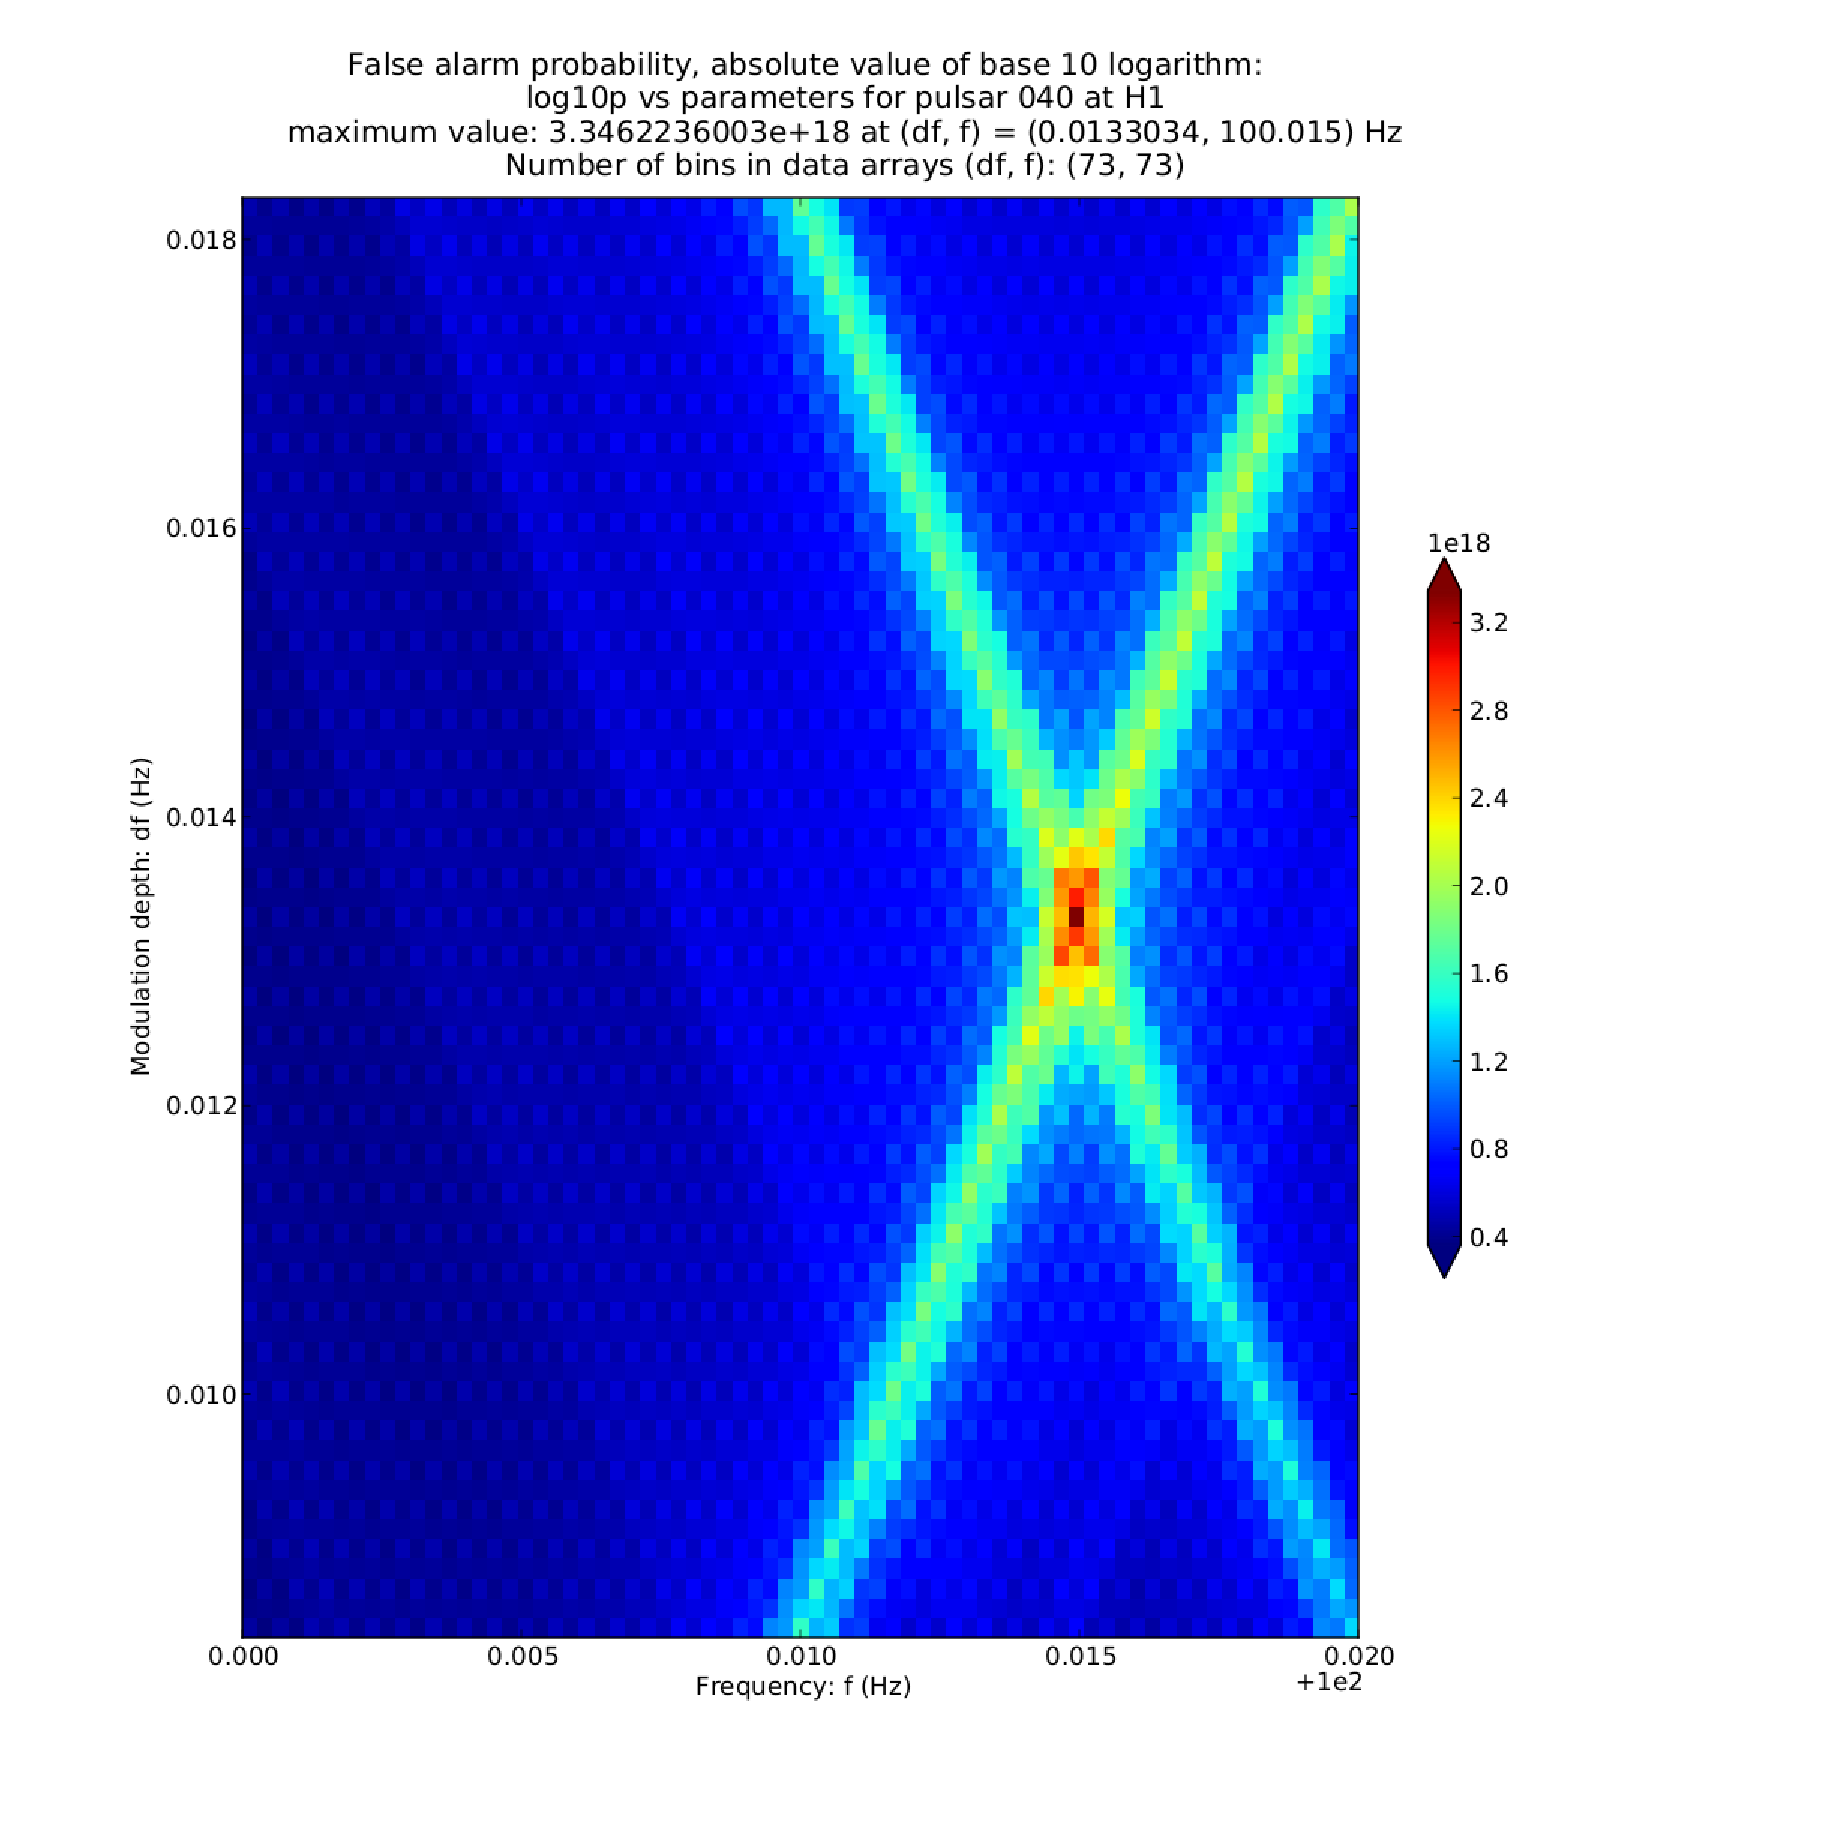
\includegraphics[width=0.8\paperwidth,height=0.62\paperheight]{Prob-4e21-on-4e24.eps}
\caption{The Davies algorithm translates $R$ statistic values for exact templates into (single-template) $p$-values, plotted on the modulation depth vs frequency plane.}
\end{center}
\end{figure}


%\end{frame}

%\section{Directed searches for neutron stars in binary systems}

%\begin{frame}{Directed TwoSpect's greater sensitivity}
\section{Directed TwoSpect's greater sensitivity}

Historical interest: the system of right ascension and declination were fixed by the time of Corpernicus, \textit{De revolutionibus orbium coelestium}~\cite{Hawking2002}.
Modern interest: searching over a wide range of right ascensions and declinations can multiply computational times for gravitational wave searches by many orders of magnitude, because each frequency GW needs to be corrected by a phase and amplitude Doppler correction unique to each sky location.
The number of distinct sky points needed is discretized by the allowed mismatch in sensitivity between points, but even a search across the LIGO frequencies requires $\mathcal{O}(10^9)$ more templates~\cite{GoetzTwoSpectMethods2011} to do an all-sky analysis rather than one at a single location. 
Note our distance from the galactic center~\cite{KerrLyndenBell1986} as 8.5 kiloparsec.




\emph{All-sky search: }parameter space $\gg10^{18}$ templates
\begin{itemize}
\item Hierachical search; incoherent harmonic sum to consolidate\\
parameter space, use templates to test interesting outliers
\end{itemize}

\emph{Directed search: }parameter space much smaller
\begin{itemize}
\item Fully template the parameter space for max sensitivity
\end{itemize}

\textbf{Scorpius X-1 (P $\approx$$ $ 68023.7 s, a sin $\iota$ $\approx1.44\pm0.18$
s):}


\[
N_{\textup{{template}}}=(f_{max}-f_{min})(2T_{coh}){\displaystyle \Sigma}_{f_{min}}^{f_{max}}(2\pi f)(4T_{coh})\frac{a\sin\iota}{P}
\]



$N_{template}\approx10^{8}$ for 3 interferometers (500 Hz band; $3\sigma$
in $a\sin\iota$)$ $
\begin{itemize}
\item Tractable to test all templates$\rightarrow$ need new methods
\end{itemize}

\textbf{Test methods in Mock Data Challenge (MDC)}
\begin{itemize}
\item TwoSpect is 1 of up to 6 algorithms looking for \\
50 ``open'', 50 ``closed/blind'' Sco X-1-like ``pulsars'' (LMXBs)
\end{itemize}
%\end{frame}

%\begin{frame}{Sky maps using exact templates}
\subsection{Sky maps using exact templates}


\begin{figure}
\begin{center}
%\protect\caption{\protect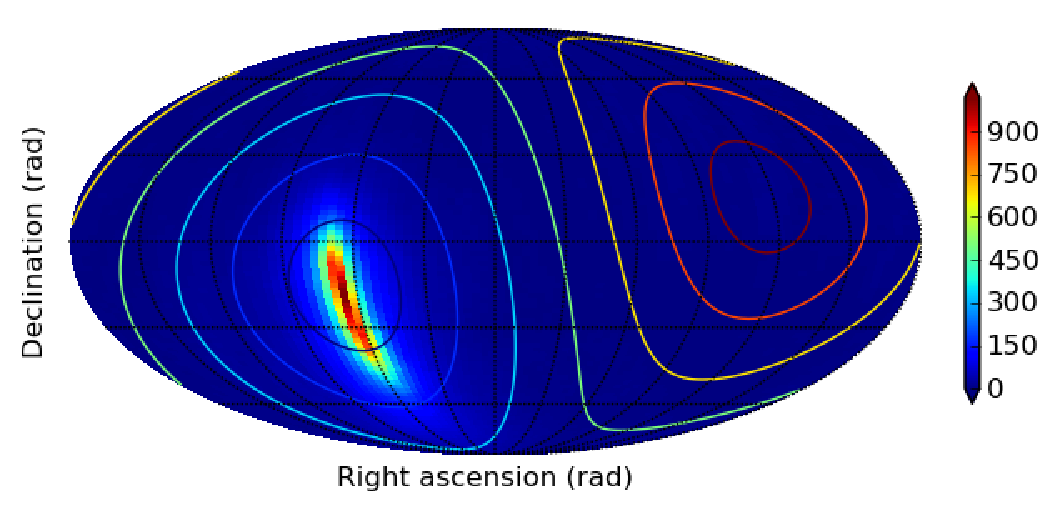
\includegraphics[width=0.4\paperwidth,height=0.2\paperheight]{maptrueH1}}
%\protect\caption{\protect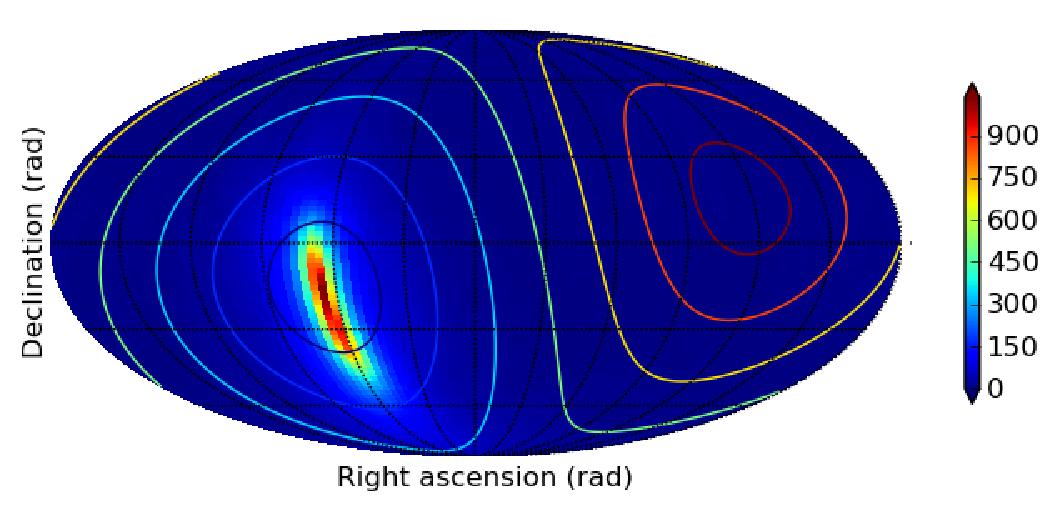
\includegraphics[width=0.4\paperwidth,height=0.2\paperheight]{maptrueL1}}
%\protect\caption{\protect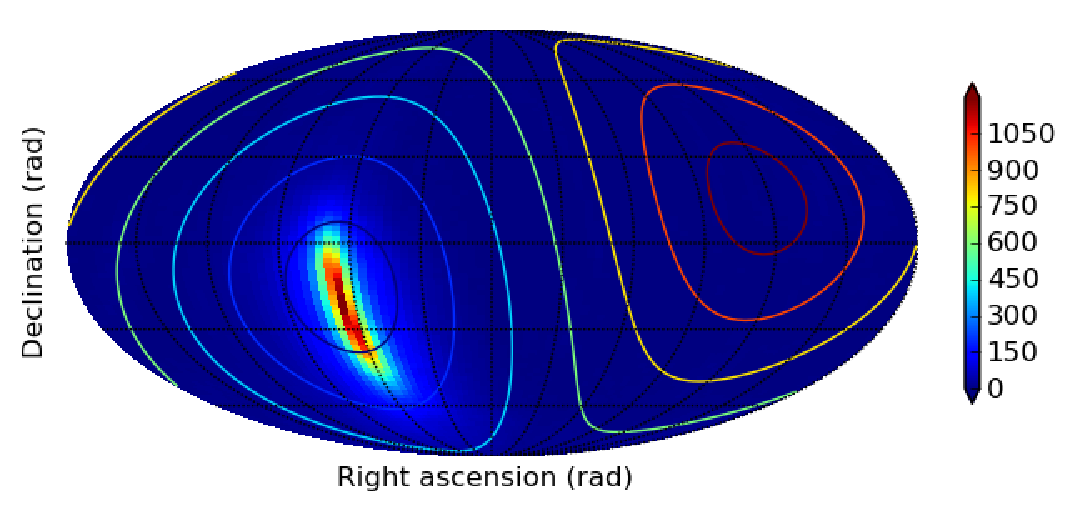
\includegraphics[width=0.4\paperwidth,height=0.2\paperheight]{maptrueV1}}
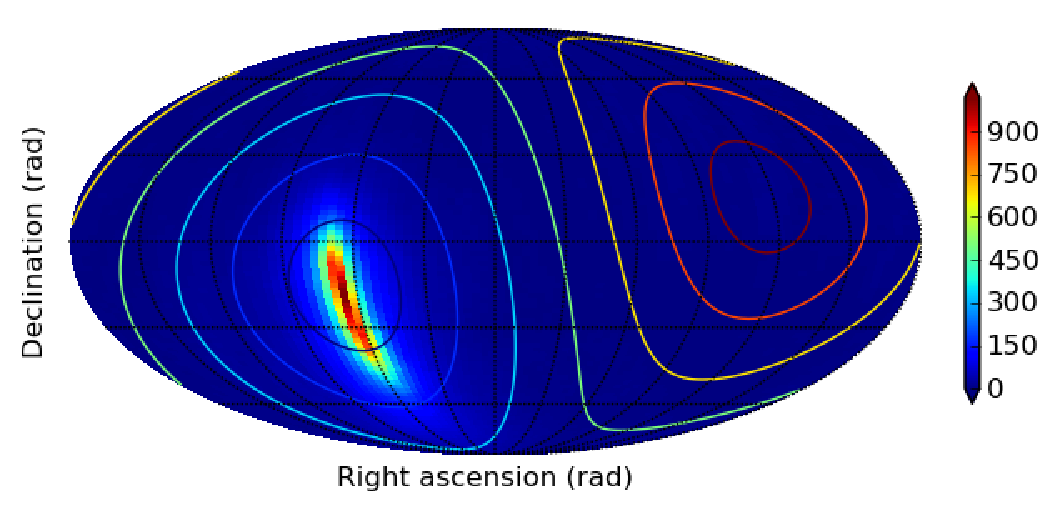
\includegraphics[width=0.6\paperwidth,height=0.2\paperheight]{maptrueH1.eps}
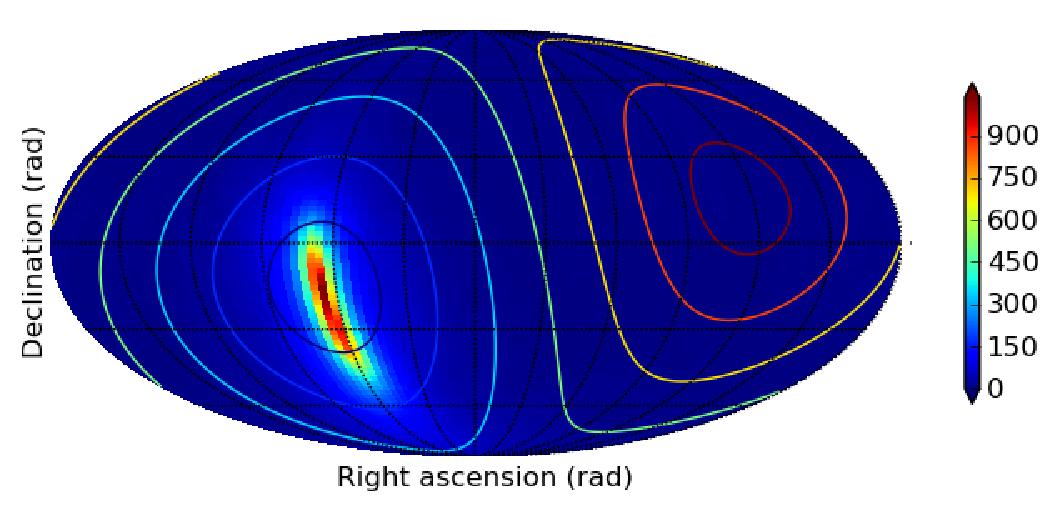
\includegraphics[width=0.6\paperwidth,height=0.2\paperheight]{maptrueL1.eps}
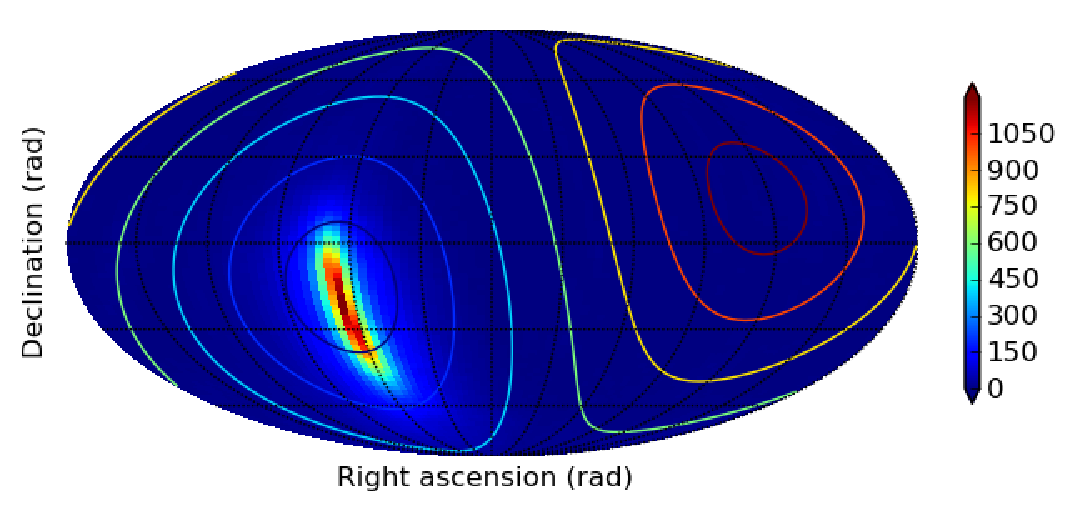
\includegraphics[width=0.6\paperwidth,height=0.2\paperheight]{maptrueV1.eps}
\caption{ All-sky maps \{H1, L1, V1\} for fixed right ascension and declination
\newline Scorpius X-1 mock data challenge pulsar 16 (101x101 templates)
}
\end{center}
\end{figure}


%\end{frame}


\section{Scorpius X-1 mock data challenge}
%\begin{frame}{Fully-templated search for Scorpius X-1}
\subsection{Fully-templated search for Scorpius X-1}


\begin{figure}
\begin{center}
%\protect\caption{\protect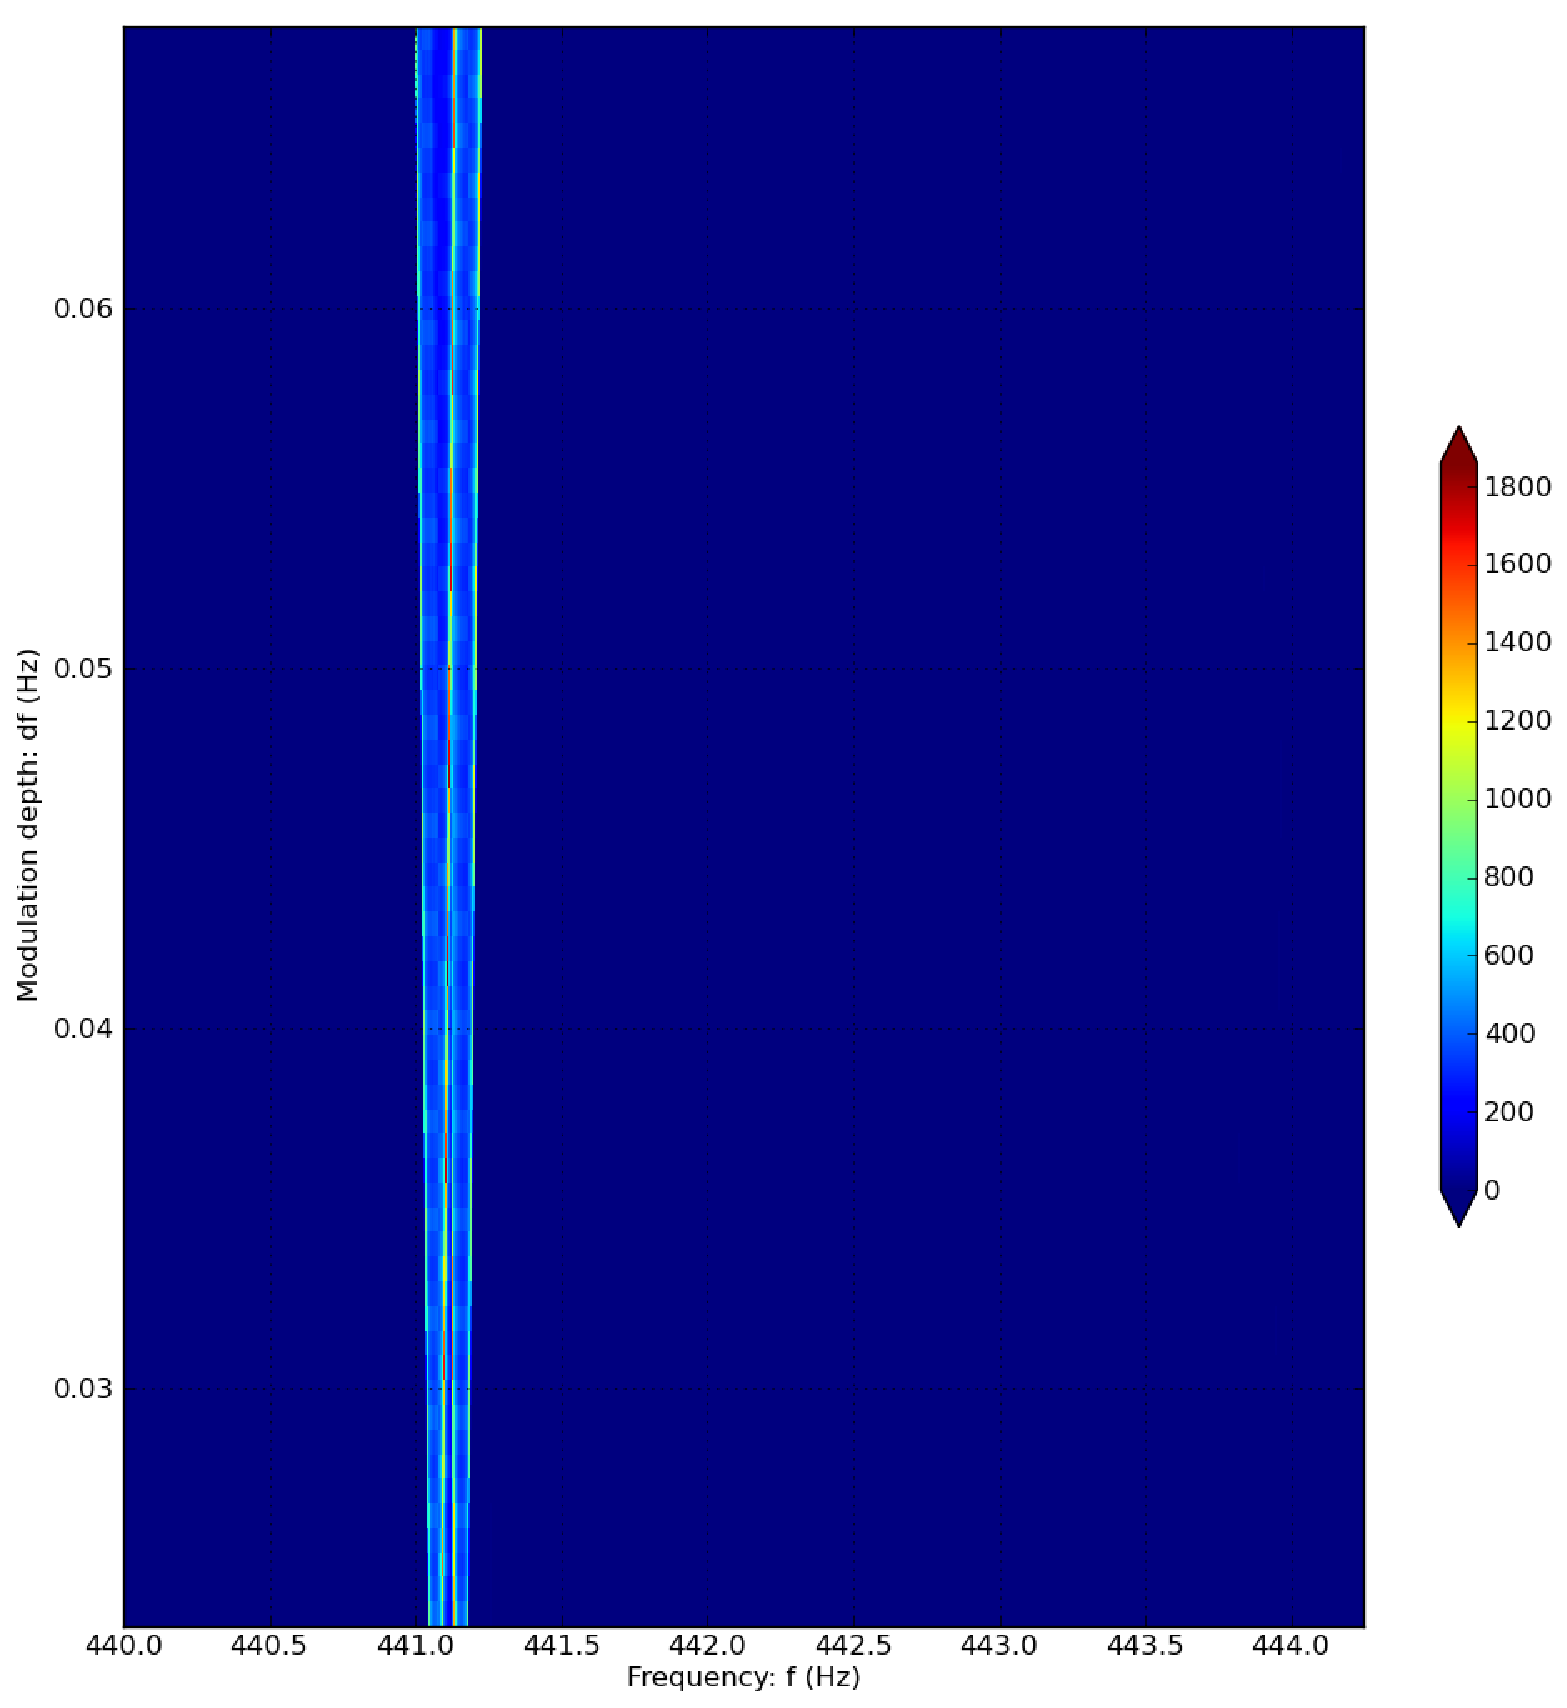
\includegraphics[width=0.8\paperwidth,height=0.62\paperheight]{bandH1-bold}}
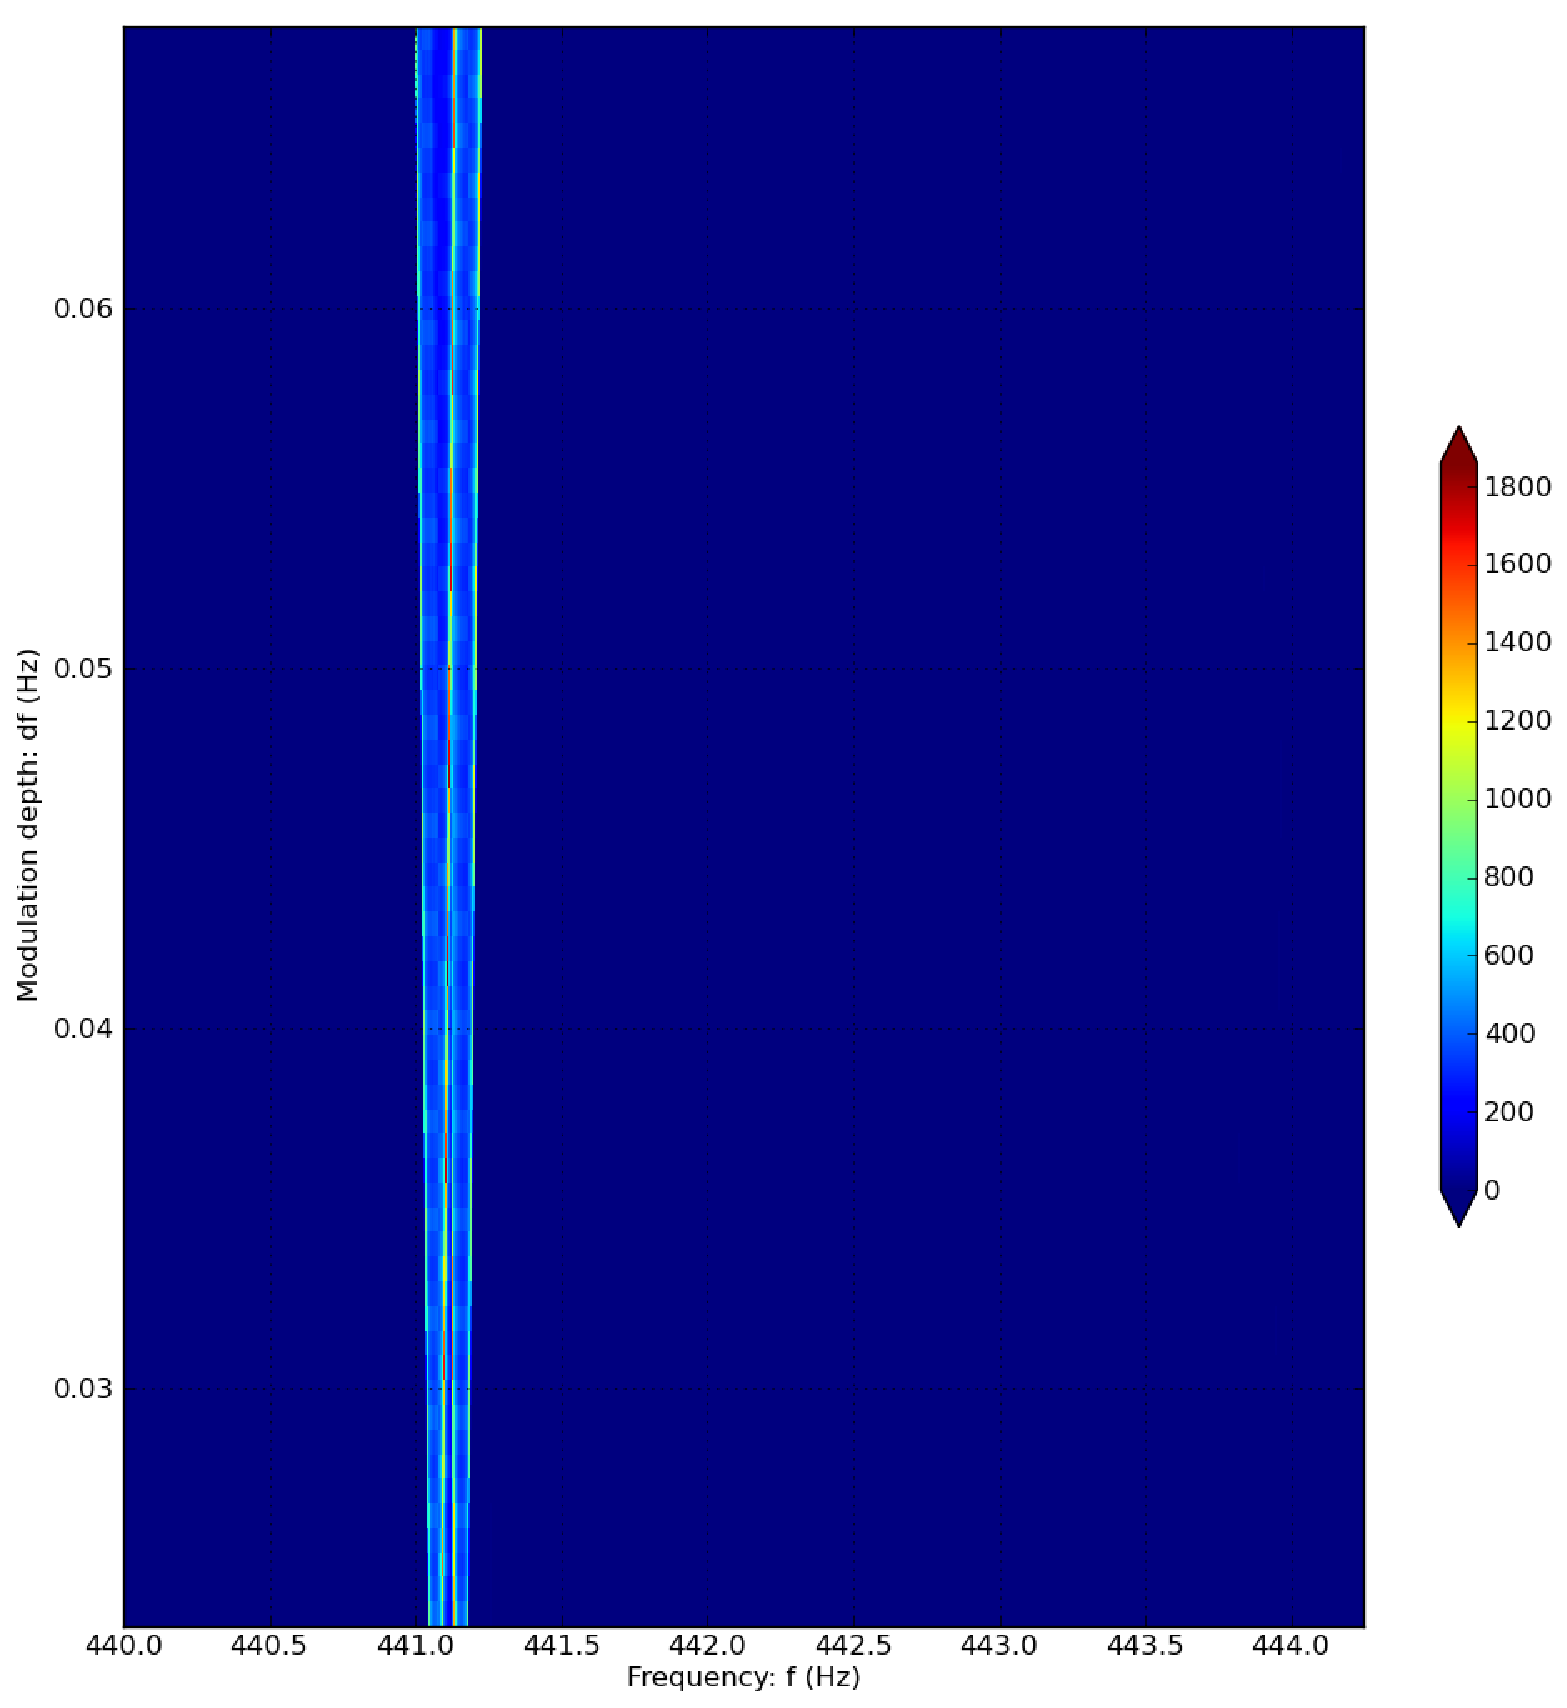
\includegraphics[width=0.8\paperwidth,height=0.62\paperheight]{bandH1-bold.eps}


\caption{
Scorpius X-1 Mock Data Challenge (MDC) pulsar 40 \{H1\}: 5 Hz band. 
The p-value (single-template, applying Davies' Method to the R statistic) in is show in this heatmap, peak in red. 
All templates are plotted on the (frequency, modulation depth) plane.
This is a relatively broadband view.
}
\end{center}
\end{figure}


%\end{frame}

%\begin{frame}{Narrow-band heat maps in parameter space}
\subsection{Narrow-band heat maps in parameter space}


\begin{figure}
\begin{center}
%\protect\caption{\protect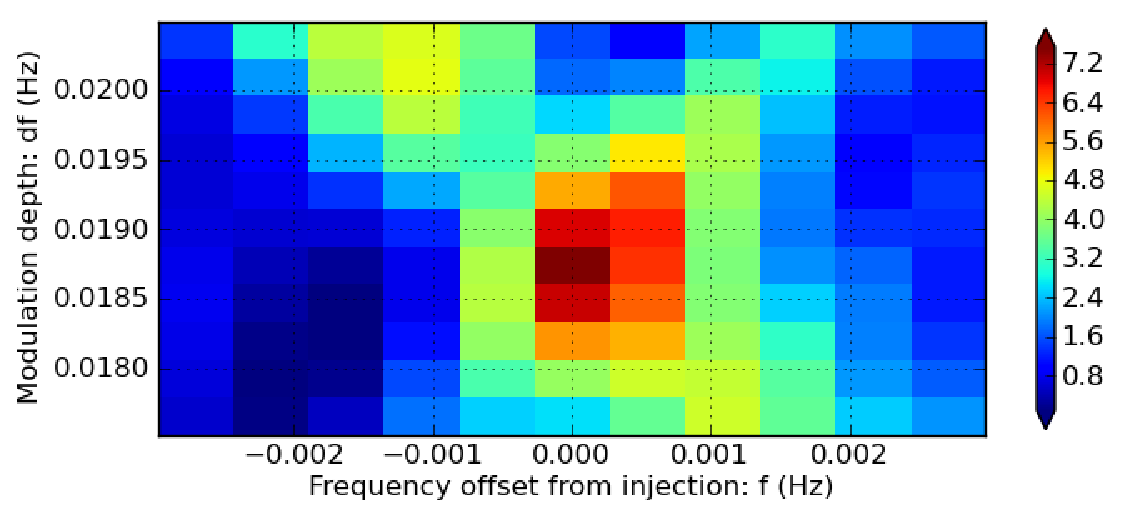
\includegraphics[width=0.4\paperwidth,height=0.2\paperheight]{heatmapH1}}
%\protect\caption{\protect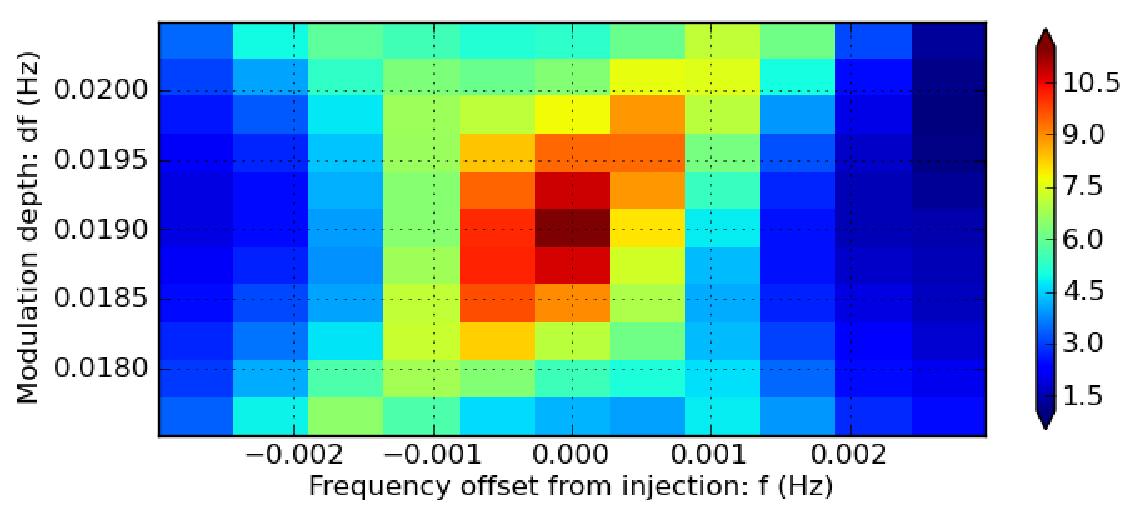
\includegraphics[width=0.4\paperwidth,height=0.2\paperheight]{heatmapL1}}
%\protect\caption{\protect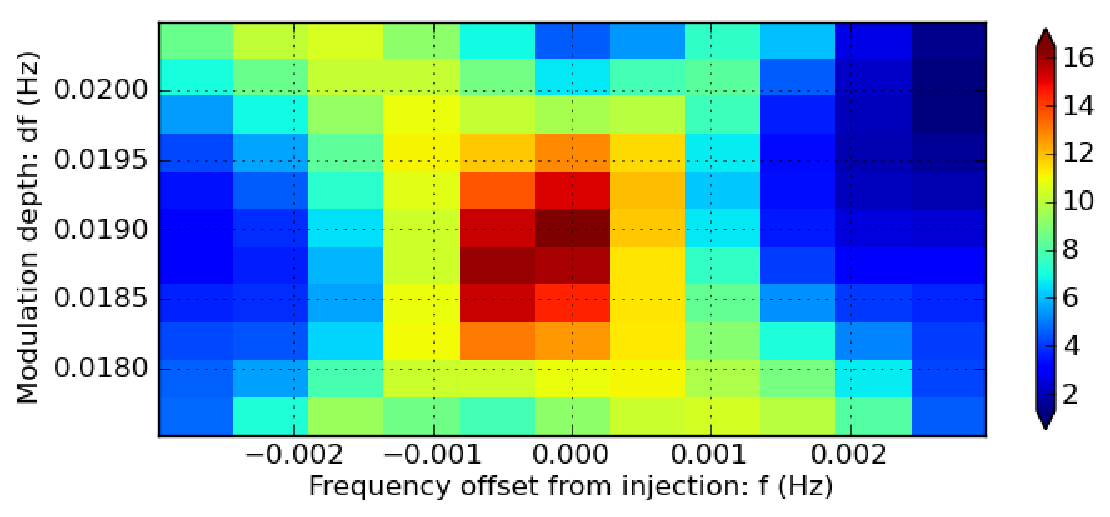
\includegraphics[width=0.4\paperwidth,height=0.2\paperheight]{heatmapV1}}
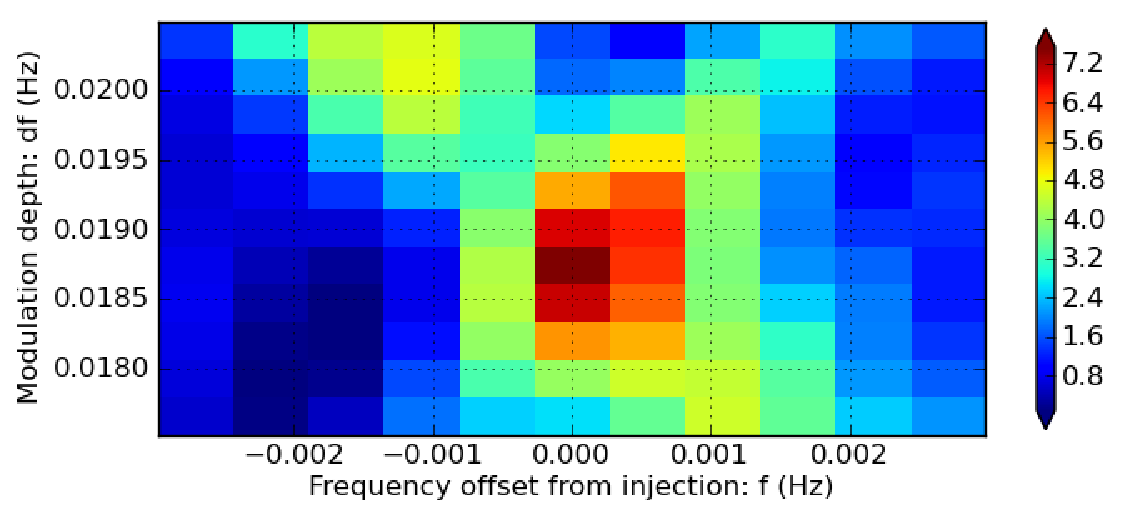
\includegraphics[width=0.6\paperwidth,height=0.2\paperheight]{heatmapH1.eps}
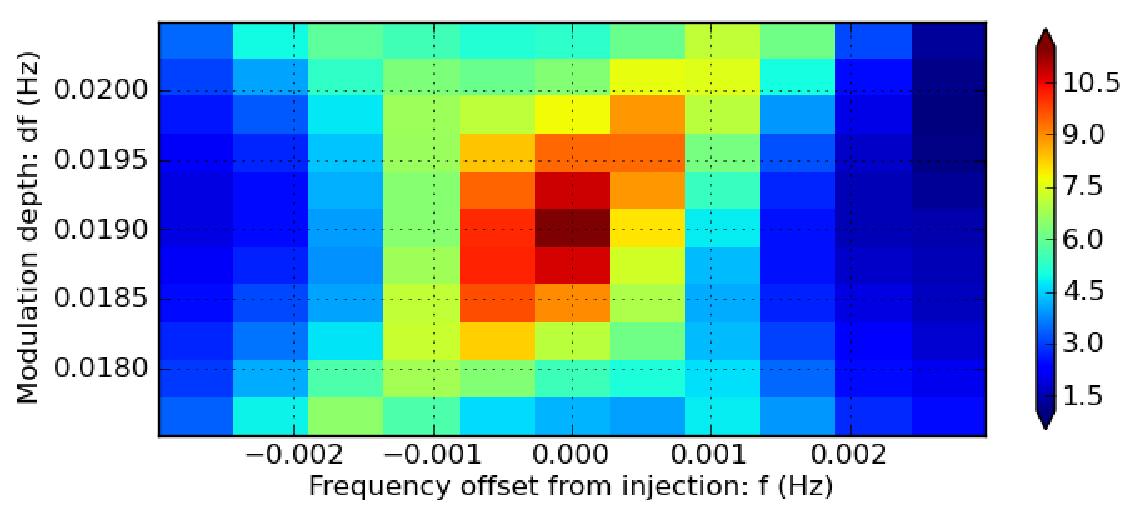
\includegraphics[width=0.6\paperwidth,height=0.2\paperheight]{heatmapL1.eps}
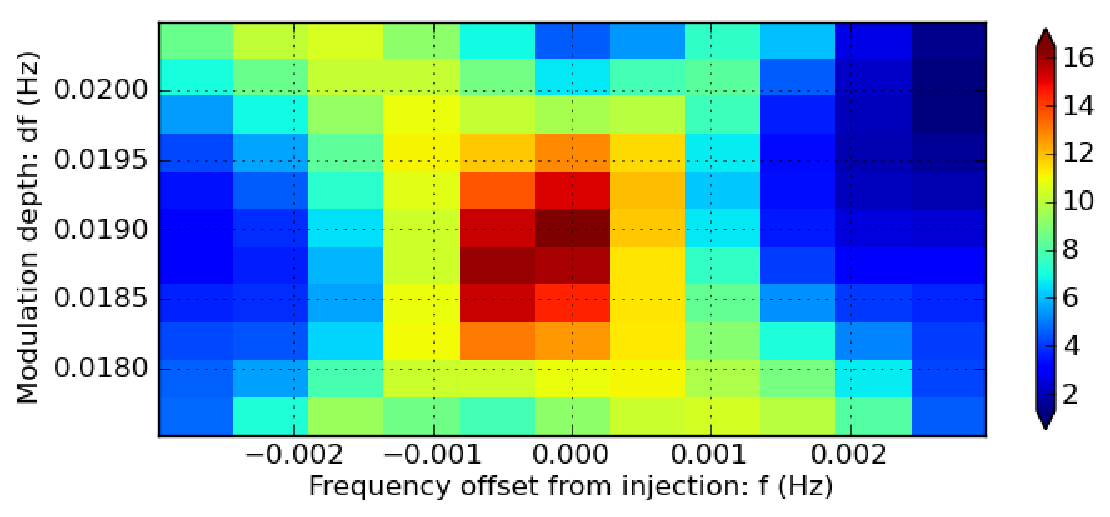
\includegraphics[width=0.6\paperwidth,height=0.2\paperheight]{heatmapV1.eps}
\caption{Heatmaps \{H1, L1, V1\} of 11x11 templates centered around
Scorpius X-1 MDC pulsar 8. 
This is a relatively narrowband view.
}
\end{center}
\end{figure}


%\end{frame}

%\begin{frame}{Wide-band heat maps in parameter space}
\subsection{Wide-band heat maps in parameter space}


\begin{figure}
\begin{center}
%\protect\caption{\protect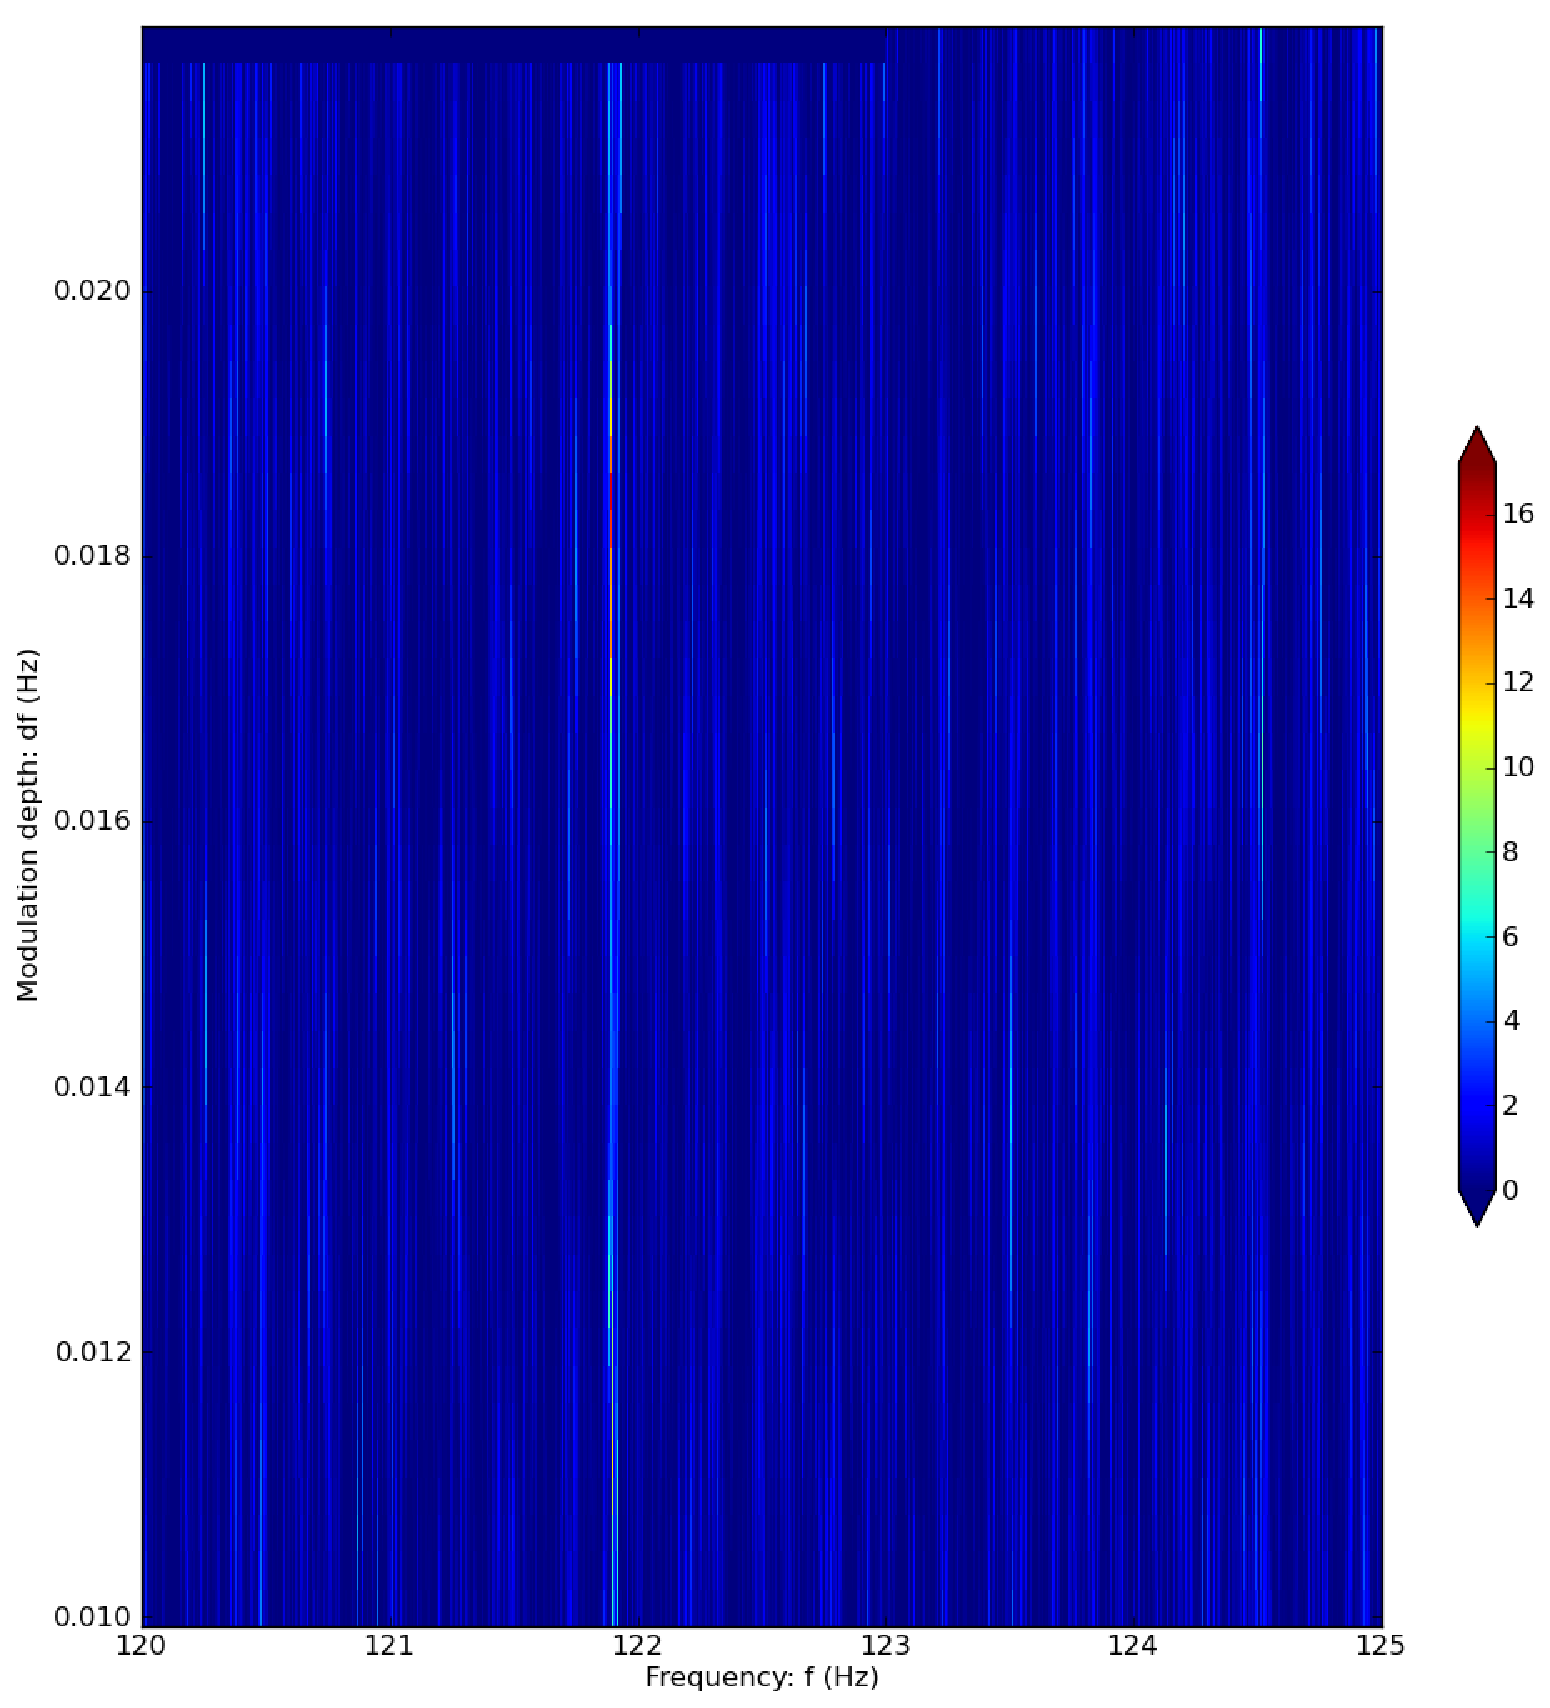
\includegraphics[width=0.8\paperwidth,height=0.62\paperheight]{bandH1}}
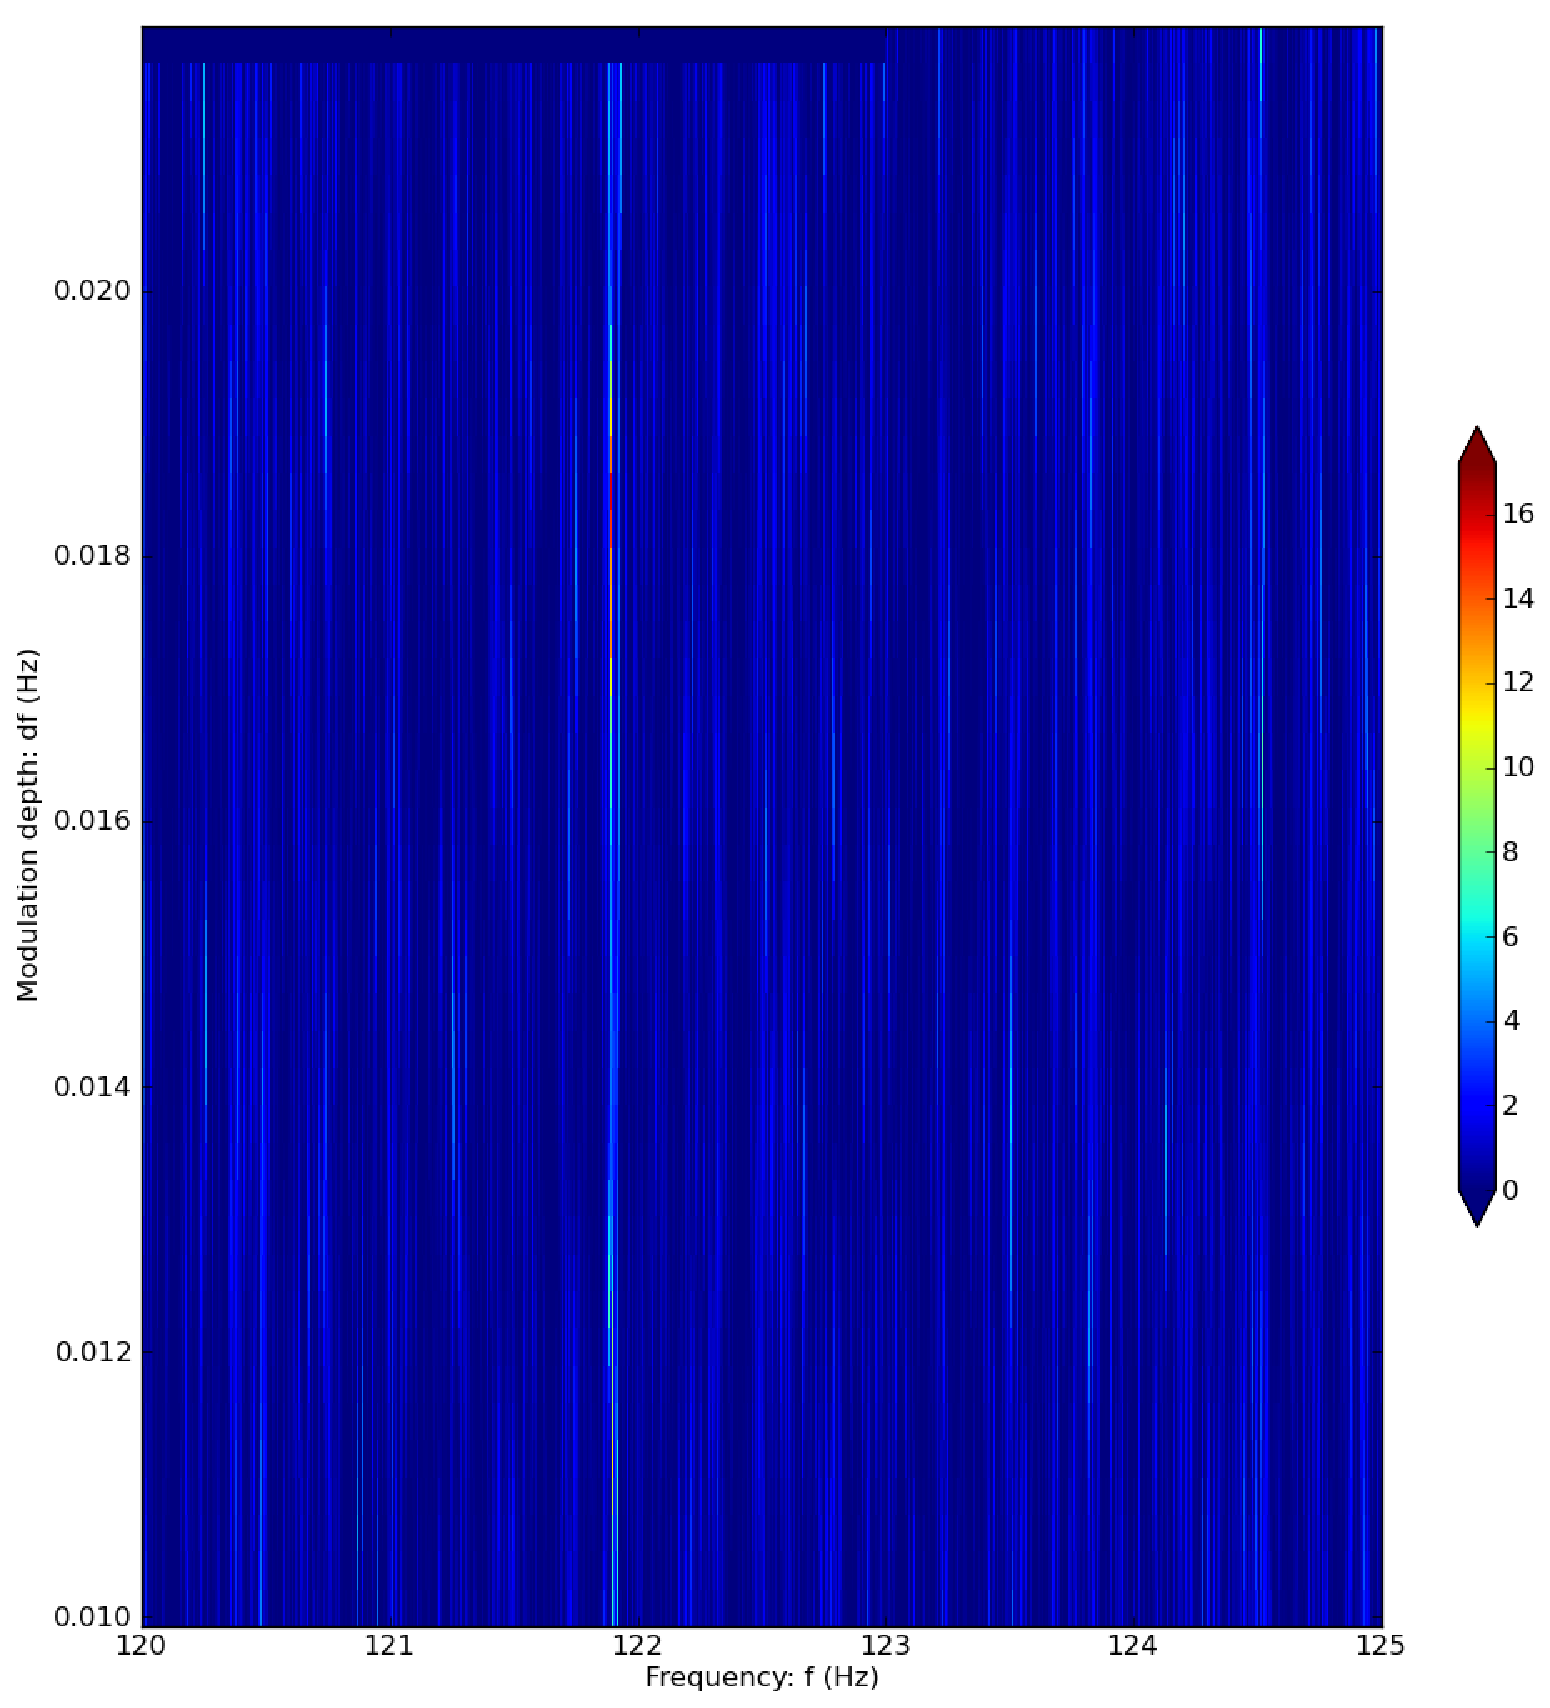
\includegraphics[width=0.8\paperwidth,height=0.62\paperheight]{bandH1.eps}
\caption{Scorpius X-1 MDC pulsar 8 \{H1\}: 5 Hz band. This heatmap shows $3.6\times10^{5}$ templates, 10-22 mHz modulation depth, 120-125 Hz frequency. The peak siignal at about (df = 0.019, f = 121.9) Hz.
}
\end{center}
\end{figure}


%\end{frame}

%\begin{frame}{Revisiting \& refining detection criteria}
\subsection{Revisiting \& refining detection criteria}


\begin{figure}
\begin{center}
%\protect\caption{\protect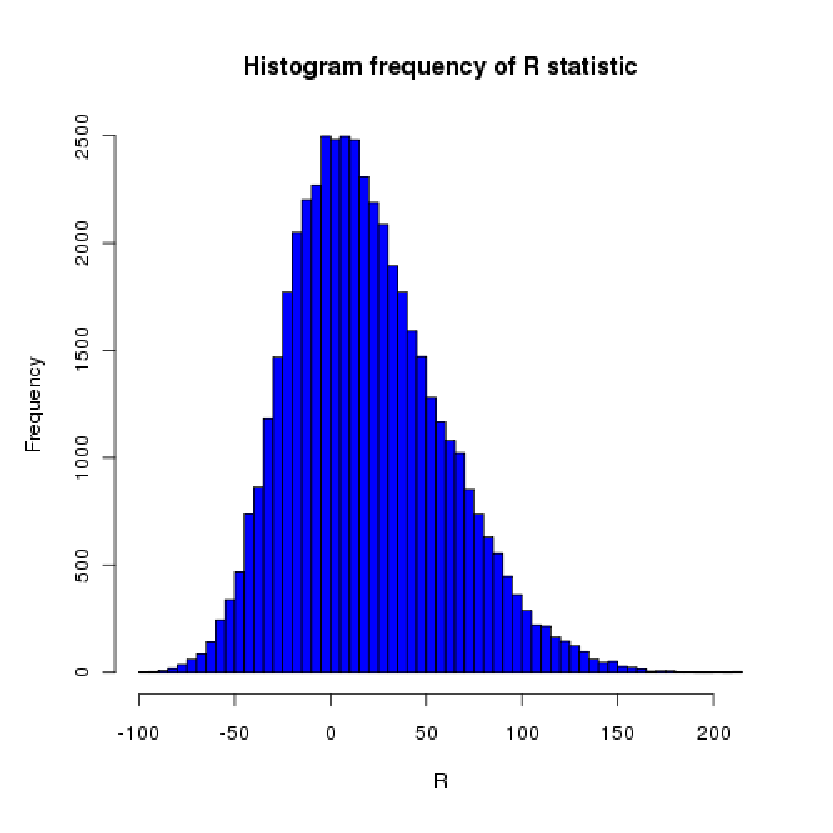
\includegraphics[width=0.45\paperwidth,height=0.45\paperheight]{StatHistRH1}\protect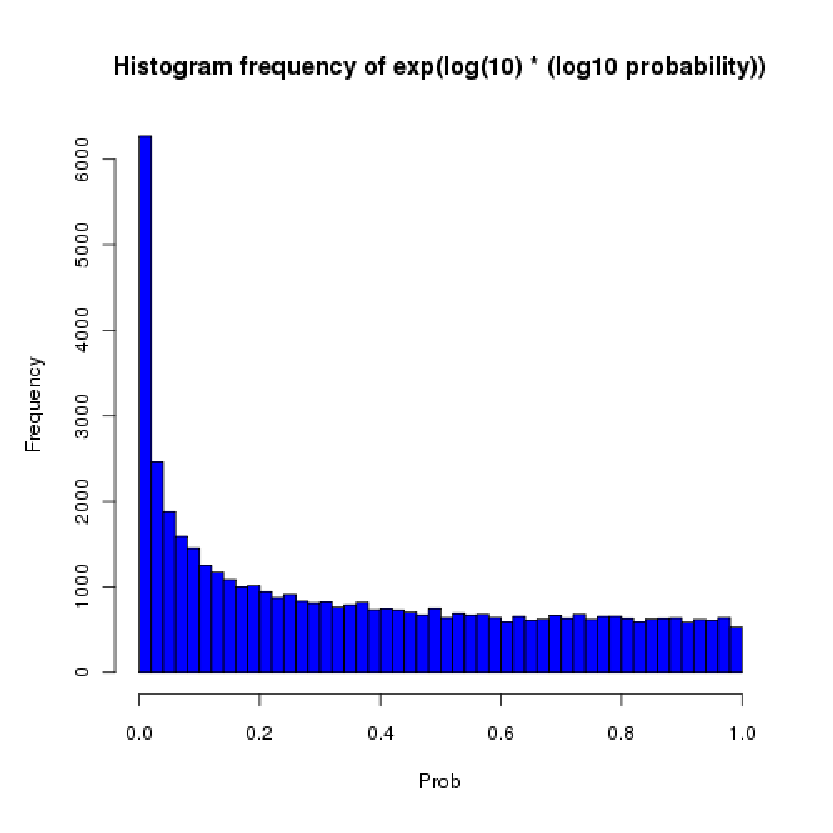
\includegraphics[width=0.45\paperwidth,height=0.45\paperheight]{StatHistProbH1}}
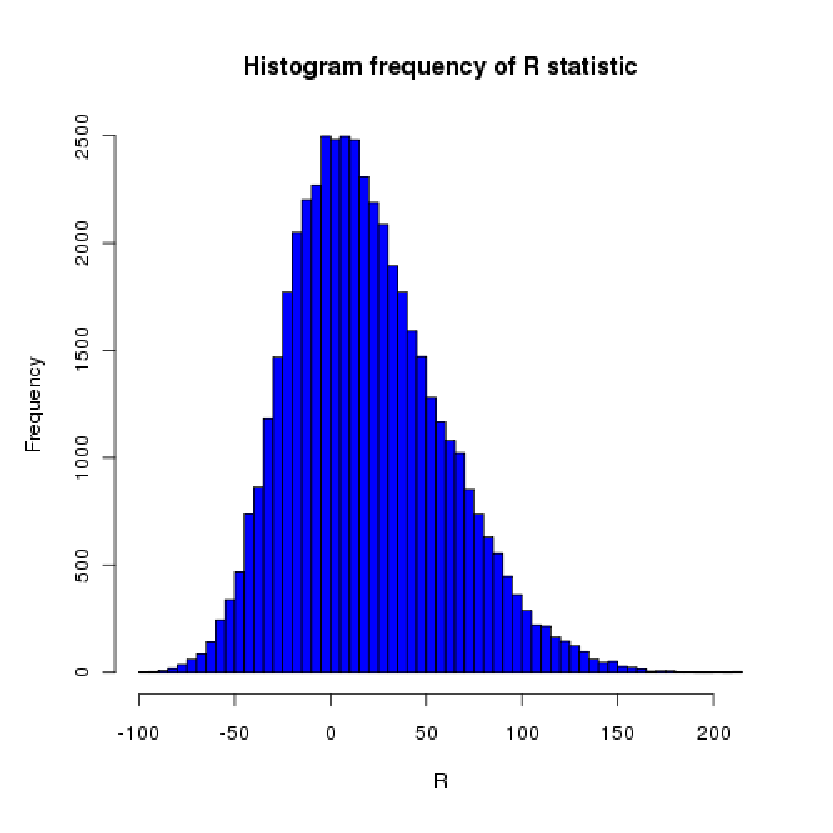
\includegraphics[width=0.6\paperwidth,height=0.35\paperheight]{StatHistRH1.eps}
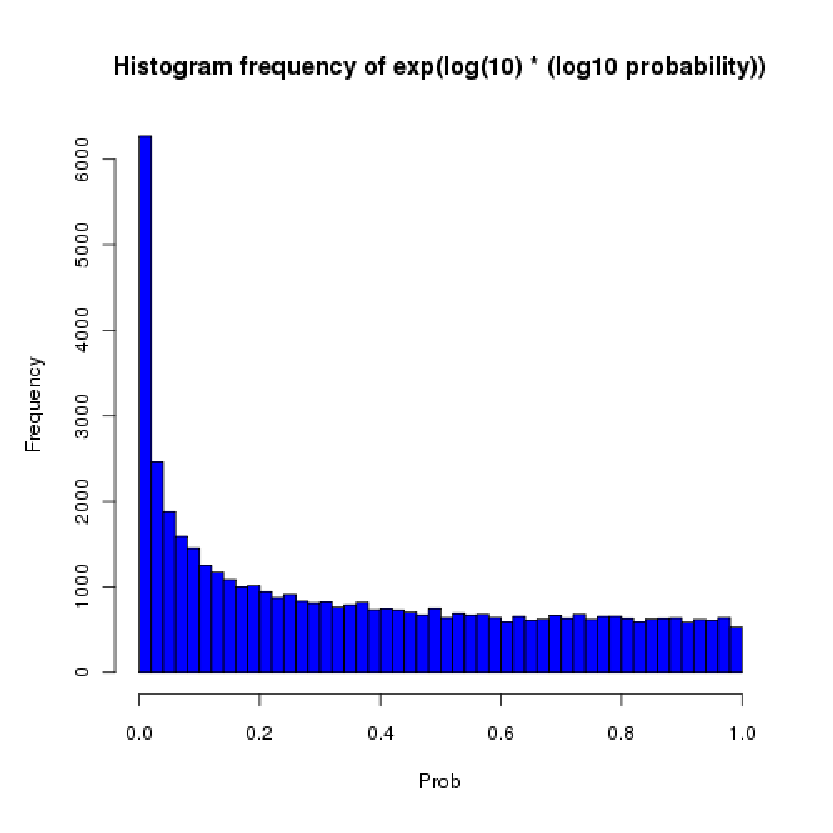
\includegraphics[width=0.6\paperwidth,height=0.35\paperheight]{StatHistProbH1.eps}
\caption{Scorpius X-1 MDC statistics. These histograms of the $R$ statistic and $p$-value distribution were part of understanding noise, temporal gap \& spectral leakage, as well as establishing a threshold p-value $\sim$ false alarm probability of 1\%.
These $p$-values are for single templates, appropriate to the all-sky search but not to a dense templated search with a large trials factor.
Here, histograms show statistics in the absence of a signal. 
The left-skew of the $p$-values is associated with gaps in the data (as is right-skew, with different gaps).
Diurnal bias in barycentering is assumed, but the correlation is not fully understood.
}
\end{center}
\end{figure}



Running TwoSpect as a directed search algorithm involves calculating
the $R$-detection statistic across the probable parameter space. 
A search is conducted with templates for each grid point in the Scorpius 
X-1 parameter space; period is known sufficient well to restrict the search
to the two dimensions of signal frequency and frequency modulation. The
grid spacing, inversely proportional to spectrum coherence time, was
chosen to allow a mismatch no more than $0.2$ in the detection statistic.
Due to known period and sky location, the incoherent harmonic sum stage
of TwoSpect, used for the all-sky search, was bypassed entirely. 

Each interferometer in the data challenge was analyzed individually for 
the detection statistic and corresponding single-template $p$-value. A set
of highest $p$-value outliers in 5 Hz bands were produced for each 
interferometer, subject to a $p$-value threshold inferred from Gaussian noise.
These sets were compared in pairwise coincidence (H1-L1, H1-V1, or L1-V1),
where coincidence required proximity within a few grid points in the 
parameter space. Any surviving outliers were classified as a detection. 

The highest $p$-value outlier in a single interferometer in that band 
yielded the estimated parameters. Uncertainties in these parameters were also
determined from unblinded injections, using method of moments for signal
frequency and modulation depth and confidence intervals for signal
amplitude. Upper limits were declared from the best estimate of the 95
percent confidence level of non-detected unblinded injected signals. The
largest uncertainty in upper limits and signal amplitude estimation derives
from the ambiguity in between true $h_0$ signal and $\cos \iota$ inclination.
This ambiguity cannot be resolved with the present algorithm and depends
partially on the assumed prior distribution of signal ampltitudes; the
uncertainty was estimated by simulation.  

TwoSpect claimed to detect 34 of 50 blinded signals and stated a flat
$4.23 \times 10^{-25}$ upper limit for the 16 non-detected signals. 


\textbf{MDC procedure}
\newline
\textit{Detection Claims}

After studying the Gaussian noise in the Scorpius X-1 MDC open data set, we were able to set thresholds for detection claims.

TwoSpect's R-statistic and p-value space on {frequency}x{modulation depth} showed significant structures, particular around loud injections, corresponding to the distribution of power into pixels by way of modulation depth, Earth's Doppler motion, and possibly spectral leakage. These regions of the open data set parameter space were excised before proceeding with the Gaussian noise study.

TwoSpect also found differences in the noise between the 360 s SFTs, used for pulsar bands above 360 Hz, and the 840 s SFTs, used for those bands below. The shorter SFTs were noisier.

After studying the effect of pairwise coincidence requirements on surviving Gaussian noise outliers, we were satisfied that we would achieve a false alarm rate of 0.01 or better by setting the following detection criteria. Note that the log10p values refer to single-template p-values, which are generally correlated with each other.

Detection criteria:

\begin{itemize}
\item each candidate must survive at least one double-IFO coincidence test, involving a pairwise comparison of single-IFO candidates to see whether they are within 1/Tsft in both frequency (f) and modulation depth (df).
\item single-IFO candidates are the up-to-200 most extreme p-value outliers in a 5 Hz band that had a log10p $\leq$ threshold, where threshold = -7.75 if f $<$ 360.0 Hz (those that used 840 s SFTs) or -12.0 if f $\geq$ 360.0 Hz (those that used 360 s SFTs).
\end{itemize}

$\rightarrow$ if there is any candidate surviving these criteria in a 5 Hz band, we mark detected, else not detected

\textit{Parameter Estimation}

Open MDC data gave TwoSpect the the ability to check its parameter estimation on the 31 pulsars detected in the open data set.

Note that the h0 reported in this section had not yet been recalibrated for either the $\cos \iota$ ambiguity due to assumed circular polarization (see subsequent section, factor of 1.74) or a systematic rescaling endemic to TwoSpect (factor of 1.11). Instead, the first step was to rescale the known h0-injected from the MDC open data table into an h-effective. This h-effective equaled $\sqrt{ ((1+\cos^2 \iota) / 2)^2 + (\cos \iota)^2 }/\sqrt{2}$ * h0-injected, the rescaling necessary to convert the strain into effective units of circular polarization strain. Any pipeline that assumes circular polarization should require a similar procedure.

We plotted the error in the h0 reported by TwoSpect versus h0-effective for the 31 open pulsars detected.


\begin{figure}
\begin{center}
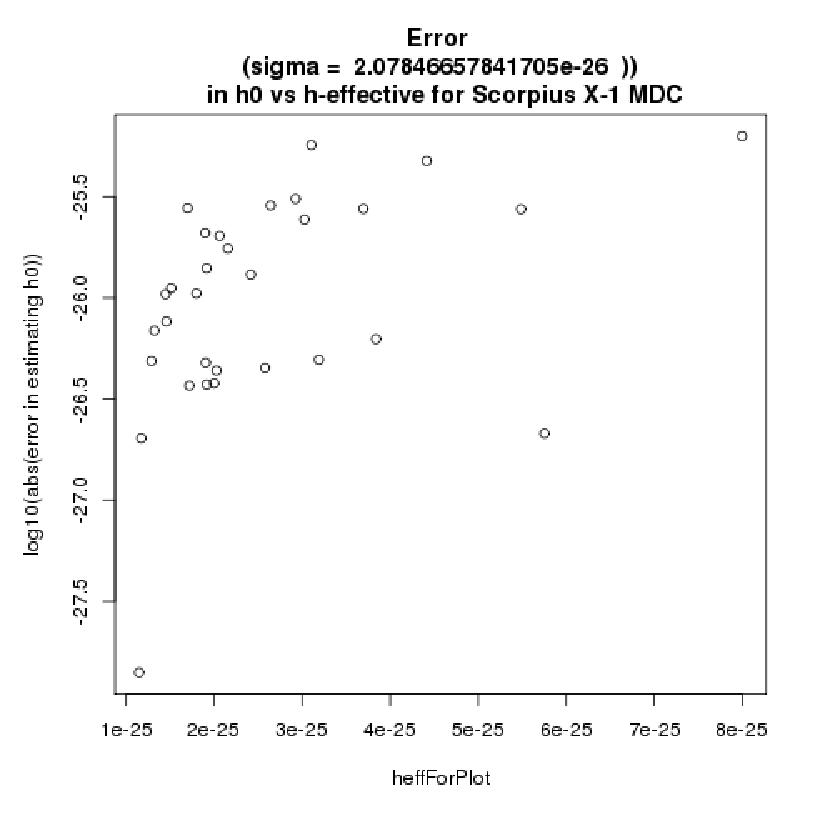
\includegraphics[width=0.3\paperwidth,height=0.2\paperheight]{detectedHerrVsHeffective.eps}
\caption{ Error in strain estimation versus circular-effective injected strain. Higher injected strain results in higher absolute errors.
} 
\end{center}
\end{figure}


This same error was also plotted vs p-value and frequency. As will be seen on the plots for error in frequency and asini, high-frequency outliers were found in the open data set. These outliers could be categorized heuristically as having f $>$ 1050 Hz and abs(log10p) $<$ 300. These 4 outliers were assigned into the \textit{loose} category, with a corresponding sigma. The remaining 27 were in the \textit{tight} category, to which we could assign a more stringent sigma. These values are reported in the header of the graphs.

Blue lines indicate the less stringent uncertainty. Red lines (on plots vs $p$-value) indicate a least squares power law regression.

\begin{figure}
\begin{center}
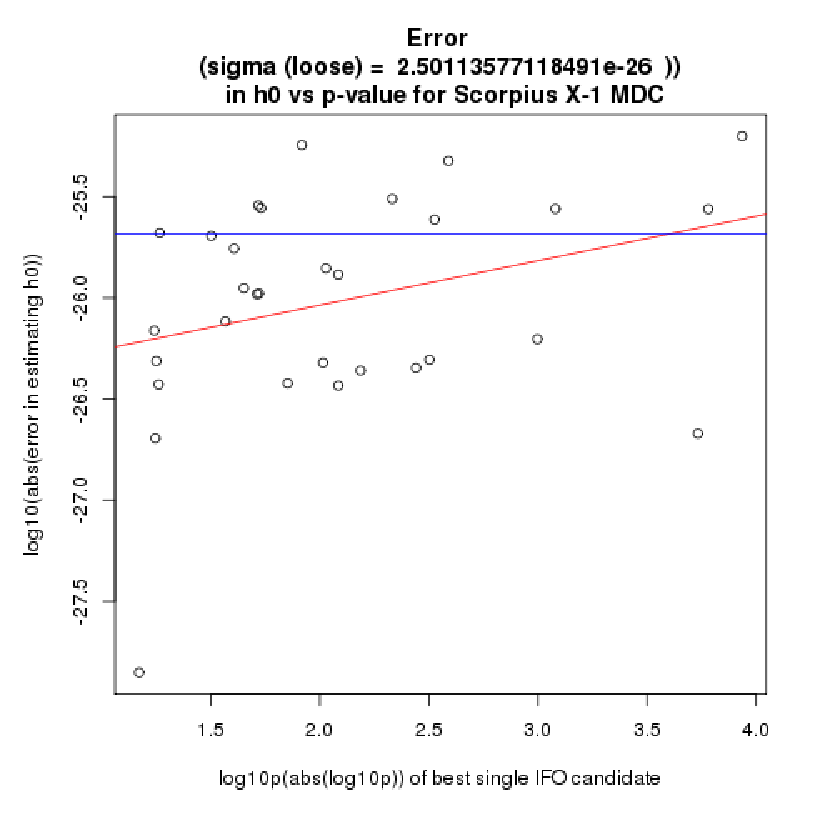
\includegraphics[width=0.3\paperwidth,height=0.2\paperheight]{Errorh0.eps}
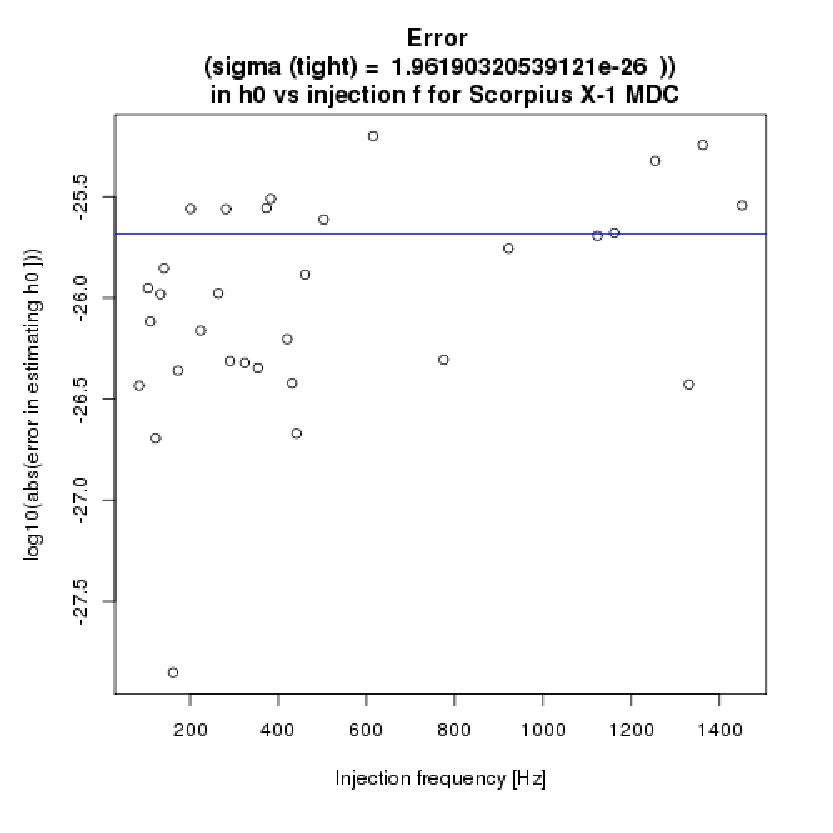
\includegraphics[width=0.3\paperwidth,height=0.2\paperheight]{Errorh0vsF.eps}
\caption{Parameter estimation: error in strain as a function of recovered $p$-value (left) and frequency (right). The strain appears broadly distriuted, without any systematic patterns.
}
\end{center}
\end{figure}


\begin{figure}
\begin{center}
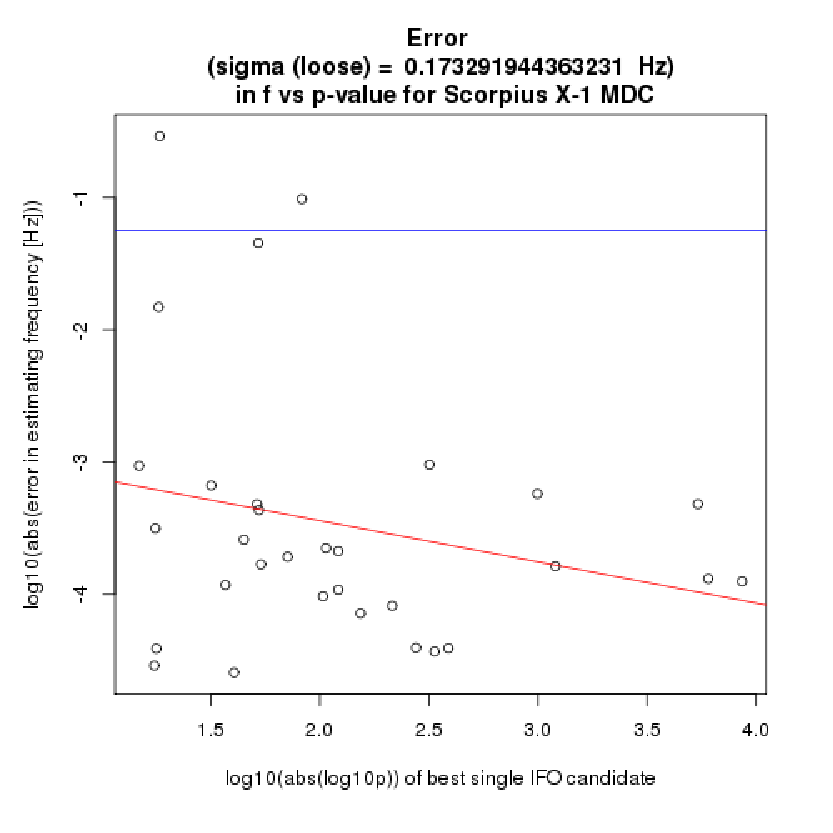
\includegraphics[width=0.3\paperwidth,height=0.2\paperheight]{ErrorF.eps}
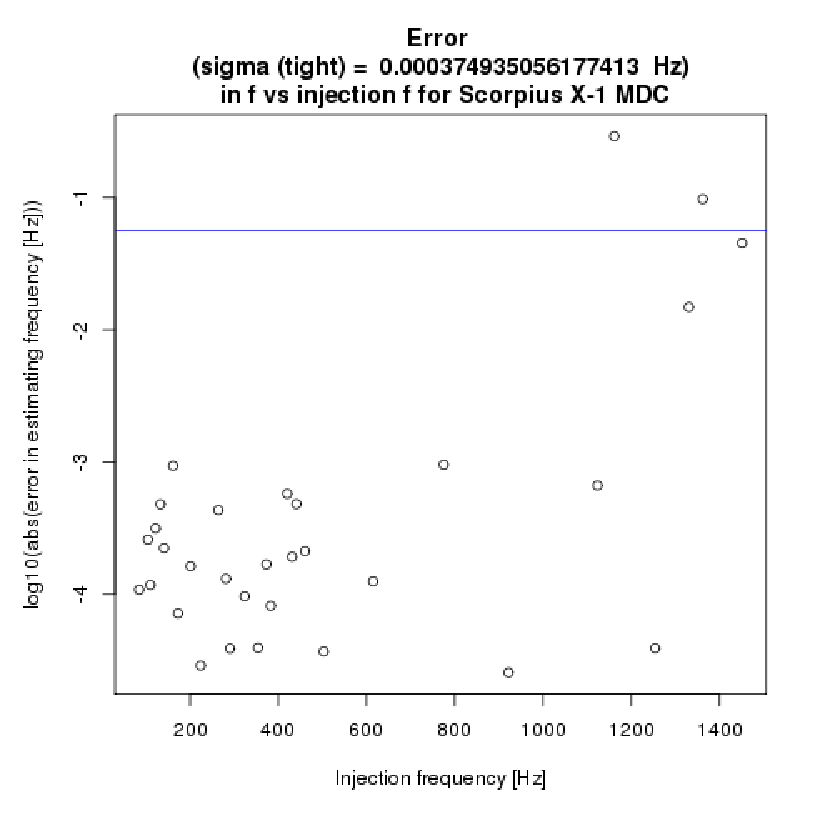
\includegraphics[width=0.3\paperwidth,height=0.2\paperheight]{ErrorFvsF.eps}
\caption{Parameter estimation: error in frequency as a function of recovered $p$-value (left) and frequency (right). A systematic, high error group can be seen, composed of four outliers in these graphs of the open data set. These defined the \textit{loose} fit category and prompted further investigation.
}
\end{center}
\end{figure}


\begin{figure}
\begin{center}
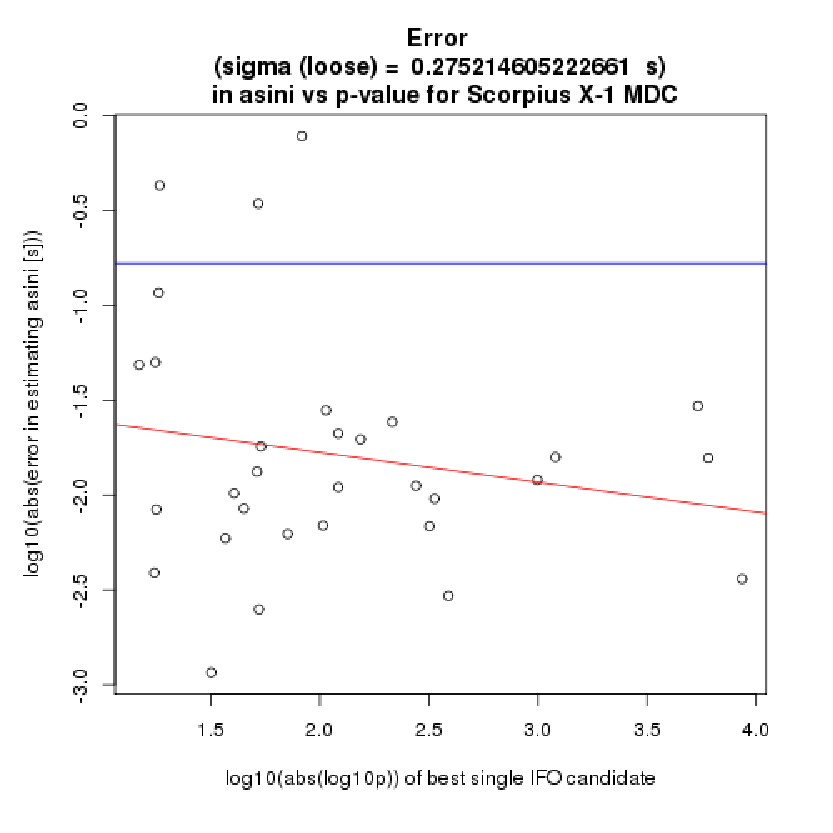
\includegraphics[width=0.3\paperwidth,height=0.2\paperheight]{ErrorAsini.eps}
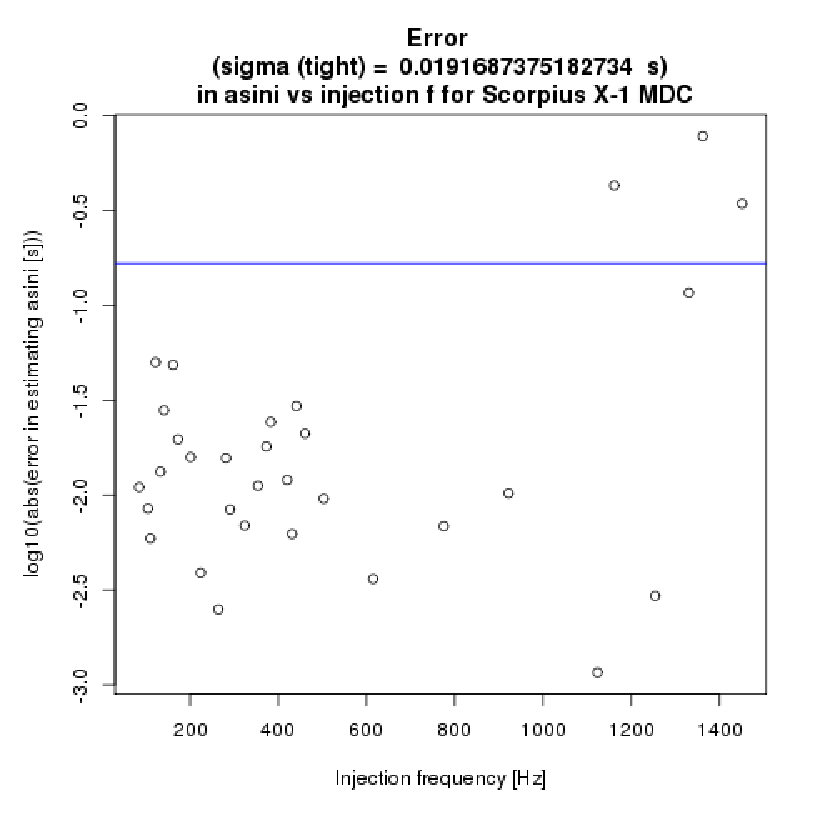
\includegraphics[width=0.3\paperwidth,height=0.2\paperheight]{ErrorAsinivsF.eps}
\caption{Parameter estimation: a sin$\iota$ (projected semi-major axis; directly proportional to modulation depth for a given frequency and period) as a function of recovered $p$-value (left) and frequency (right).
Here the same \textit{loose} outliers suffer large errors.
}
\end{center}
\end{figure}


\textit{Upper Limits and Detection Efficiency}

Upper limits and detection efficiency were also calculated using data in the open pulsar set.

For detection efficiency, we calculated the h-effective for the 31 detected and 19 non-detected pulsars and found the average detection rate in bins according to h-effective. These bins were non-uniform in size due to the interest in finding the 95\% detection efficiency point despite the paucity of statistics (only 50 pulsars total). Binomial uncertainty was also calculated and subtracted, by bin. The 95\% level is very approximately about 3$\times 10^{-25}$ (again, without the corrective factors of 1.75 and 1.11) but is imprecise to judge using this method.

\begin{figure}
\begin{center}
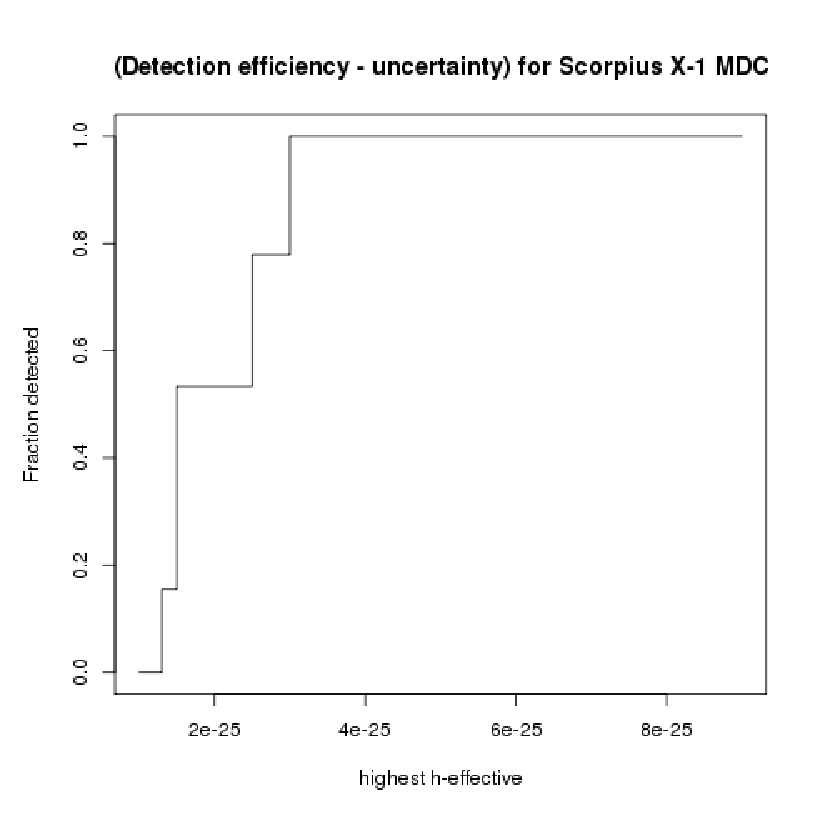
\includegraphics[width=0.3\paperwidth,height=0.2\paperheight]{detectionVsHeffective.eps}
\caption{ Open pulsar detection efficiency curve.
Because only 50 pulsars were in the open set, this curve is relatively-poorly defined -- the binning has been chosen to give the most accurate representation based on the chosen thresholds.
The curve is the worst case, equal to the efficiency minus the binomial uncertainty.
}
\end{center}
\end{figure}


Consequently we plotted the distribution of recovered h0 versus injected h0-effective (the error of which is shown above, for detected pulsars). Color-coding red pulsars as non-detected, blue as single pairwise detection, and green as triple pairwise detection, we identified a shelf of non-detected pulsars that was 95\% contained by an upper limit about 2.19$\times 10^{-25}$. This number, when corrected, yielded the upper limit of 1.74*1.11*2.19$10^{-25} = 4.23\times 10^{-25}$ for TwoSpect.

\begin{figure}
\begin{center}
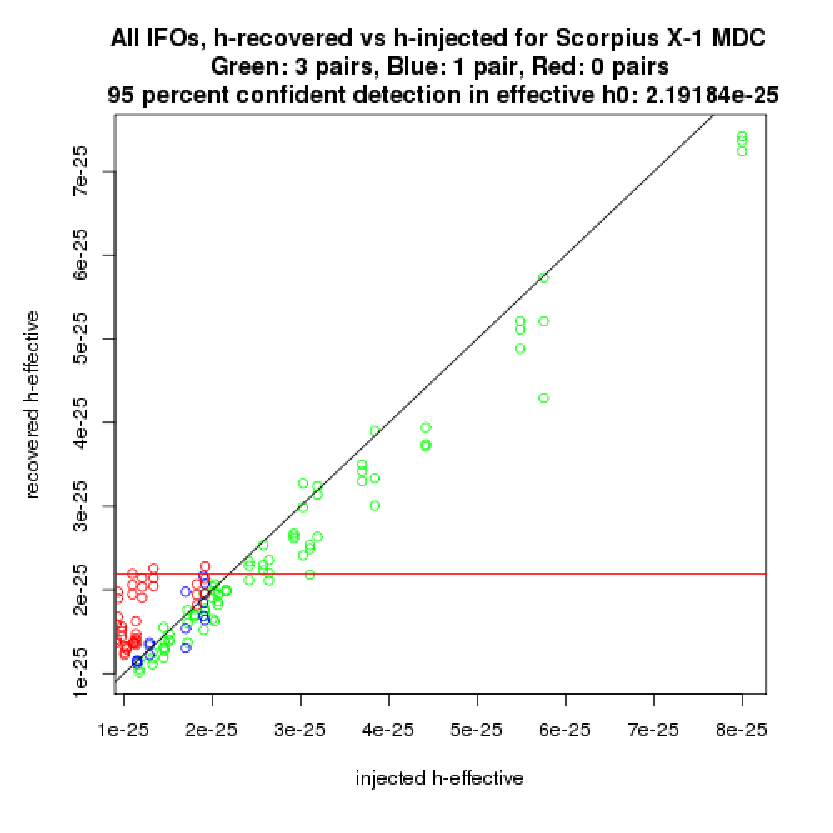
\includegraphics[width=0.3\paperwidth,height=0.2\paperheight]{HrecoveredVsHeffectiveFullUL.eps}
\caption{Detections and upper limit determination.
Depending on whether a injection was seen in three, one, or no detectors, it was assigned a color-coded circle and plotted in recovered strain versus effective circular strain injected.
The unity-slope line is shown to ascertain whether a further rescaling factor was needed (it was: constant 1.11).
The zero-slope line is shown to indicate the ninety-five percent confidence upper limit.
}
\end{center}
\end{figure}


Further injection studies should show how this upper limit varies with frequency as injected h0, but at the time of the MDC, we did not feel confident in extrapolating this relationship.
\newline
\textit{$\cos \iota$ Ambiguity}

$\cos \iota$, the cosine of the inclination angle of the pulsar, casts an ambiguity over the determination of h0. For TwoSpect, which assumes circular polarization, the true value of h0 will indeed be as reported if cos iota = 1, but will be greater if cos iota is less (i.e., the gravitational wave is elliptically polarized). In the case of linear polarization, h0 will be $2^{3/2}$ times larger than reported.

While an analytical calculation of the expectation value of the correction factor is easy, it will not easily take into account the circular bias of detected signals. That is, a pipeline will tend to see a slightly greater proportion of signals that are more circularly polarized, because the effective h0 of those signals is greater. This "circularizes" the correction factor in a way dependent on the detection efficiency of the pipeline and the assumed prior distribution of pulsars. Although the effect is relatively minor, we decided to simulate it because the size of the effect was unknown at the time.

In this simulation, 2 million pulsars were generated with h0 between 3$\times 10^{-26}$ and 3$\times 10^{-24}$ (a rough guess at the scope of the MDC) with a distribution of 1/h0.

We made a toy model of our detection efficiency, assuming no pulsars were detected below 1$\times 10^{-25}$ effective, all were above 3$\times 10^{-25}$, and the fraction detected was linear in h0 between those values.

\begin{figure}
\begin{center}
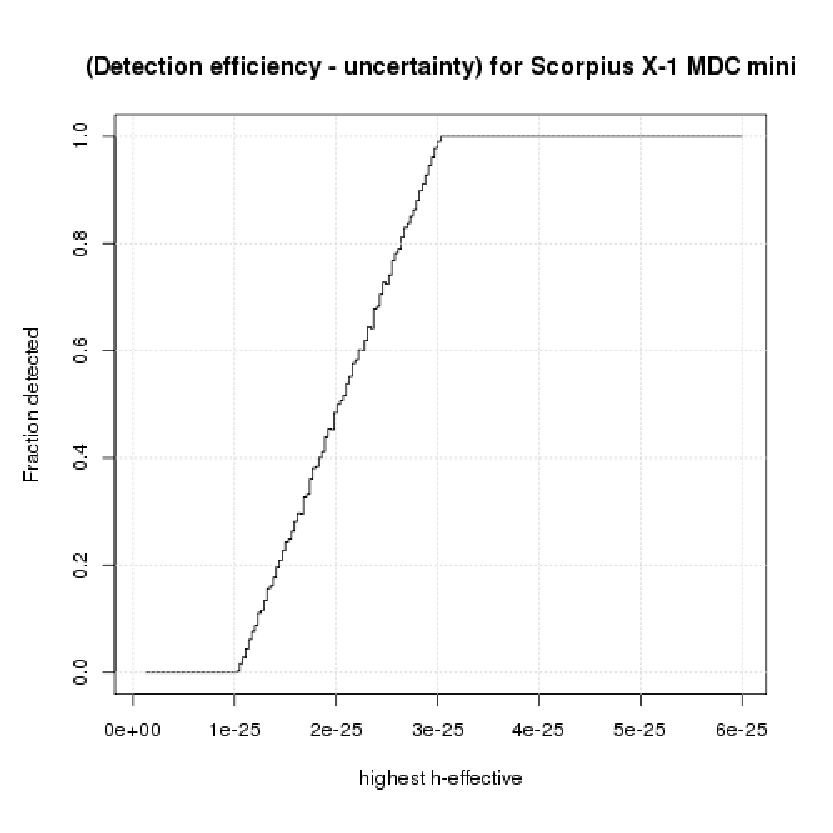
\includegraphics[width=0.3\paperwidth,height=0.2\paperheight]{PlotHeffDistH0DetectionEfficiency200breaks.eps}
\caption{ Simulated detection efficiency curve. Because the cos $\iota$ ambiguity simulation require a priori model of detection efficiency, we described it simply. Here, no detections were claimed below $1\times 10^{-25}$, all were detected above $3\times 10^{-25}$, and the probability of detection rose uniformly on the intervening interval.
}
\end{center}
\end{figure}


Together with a uniform cos iota distribution on [-1, 1], this led to a trapezoidal distribution of recovered, detected h0 values with a curved lower (left) edge:

\begin{figure}
\begin{center}
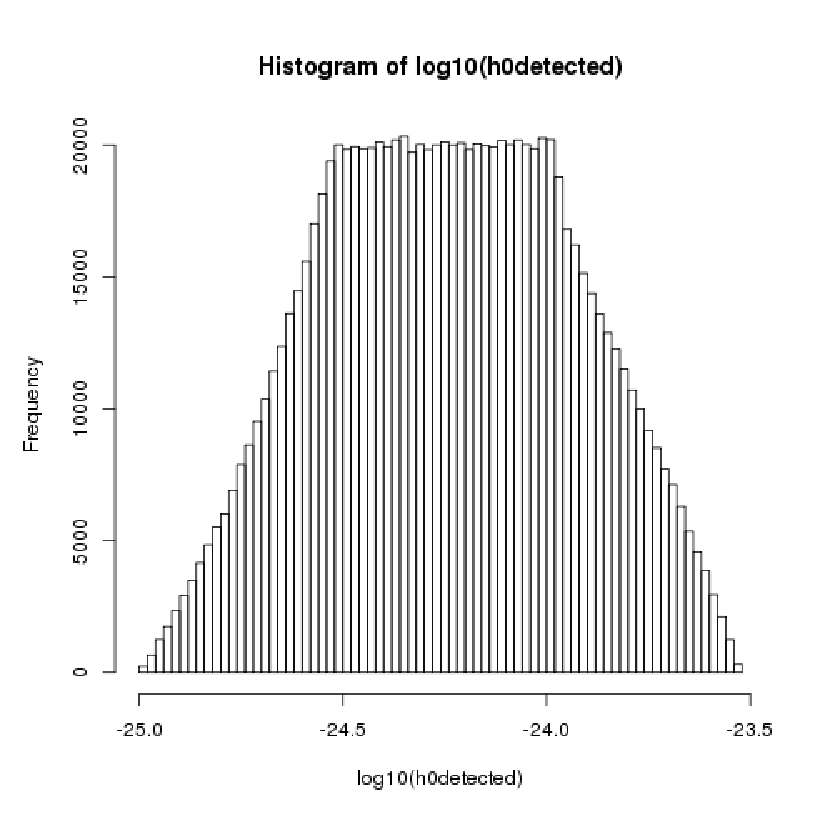
\includegraphics[width=0.3\paperwidth,height=0.2\paperheight]{PlotHEffDistH0Detected.eps}
\caption{Distribution of 2 million simulated stars, strain between $3\times 10^{-26}$ and $3\times 10^{-24}$ under a log-uniform distribution, following application of cos $\iota$ and detection efficiency cuts.
}
\end{center}
\end{figure}


The upper end of the distribution (right side of the trapezoid) was excluded because we are trying to find the average bijective mapping (slope) f: (detected h0) $\rightarrow$ (true h0), and including detected h0 $>$ 1$\times 10^{-24}$ meant that we were failing to see the complete injected h0 space. There was f$^{-1}$: (true h0) $\rightarrow$ (detected h0), but not f. More plainly, suppose we looked at a detected h0 reported as 1.5$\times 10^{-24}$, and that our average corrected factor had been calculated to be 2.5 (it was not) -- this would imply that the true h0 was 3.75 $\times 10^{-24}$ -- but this would be outside the domain of the simulation, so there would be no way to check it. The analogous problem should not happen at the lower end of the distribution (left side of the trapezoid).

In turn, we looked for the relationship between the recovered h0 of this "detected" distribution and the corresponding original, true h0. The slope would give us the conversion factor. The first attempt was to grid the {detected h0}x{true h0} space into 2D pixels. This was suggestive, and yielded the following regressed slope:

\begin{figure}
\begin{center}
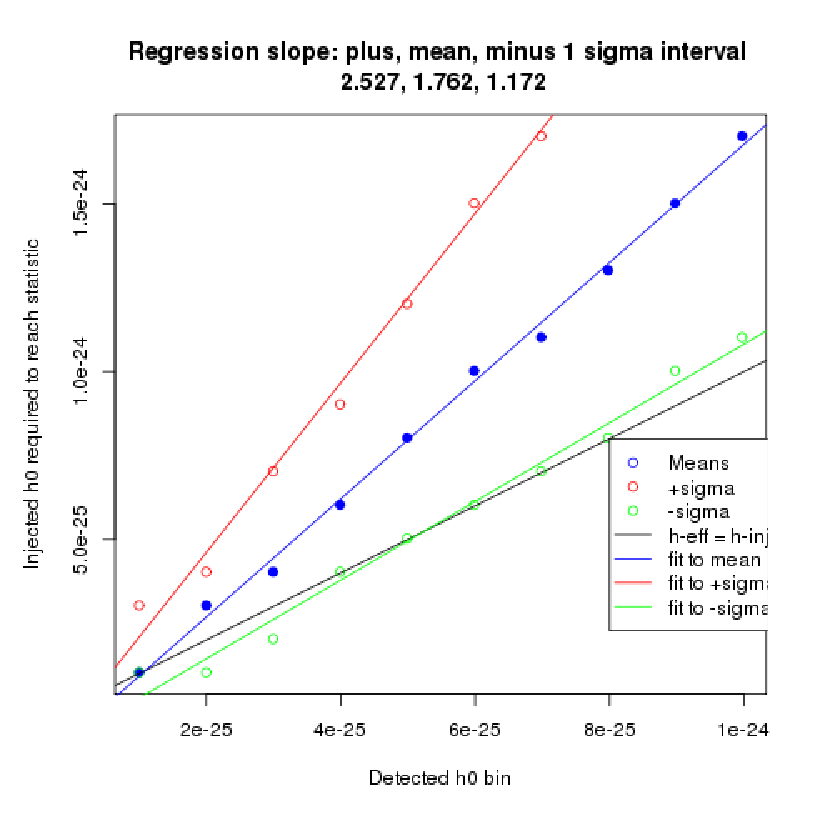
\includegraphics[width=0.3\paperwidth,height=0.2\paperheight]{PlotHeffVsH0TrueRegressions.eps}
\caption{Regression using grid. By binning the simulated stars on the true strain vs detected (recovered) strain plane, an accurate mean slope for the $\cos \iota$ correction was ascertained. It had to be modified downwards by the equivalent of one bin, to 1.74. However, the one sigma thresholds proved inaccurate, probably due to noise fluctuations.
}
\end{center}
\end{figure}


There is a systematic bias in the grid method, both by one pixel (hence why the mean was adjusted downward to 1.74) and in the associated uncertainties. Plotting these uncertainties on the distribution of {detected h0} vs {true h0} shows how wide those error bars are.

\begin{figure}
\begin{center}
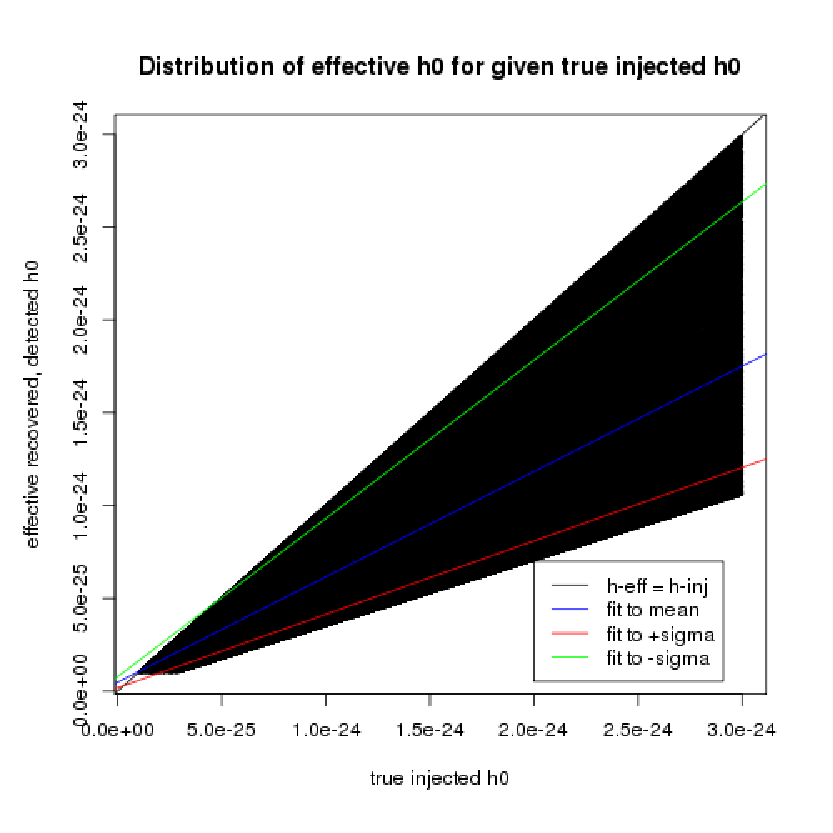
\includegraphics[width=0.3\paperwidth,height=0.2\paperheight]{PlotHEffVsH0TrueWithLines.eps}
\caption{Simulation with fit lines as given by the bin-method regression.
}
\end{center}
\end{figure}


This bias is likely due to sampling: numerical fluctuations in the grid method made it unstable at the 2 million pulsar level, especially toward the high h0 end of the distribution. Instead, we manually adjusted a $\pm \sigma$ until the CDF encompassed the appropriate 68\% confidence interval, finding a sigma in the slope of 0.37 with a mean slope of 1.74. The reason for the aforementioned restriction of the plot to h-effective $<$ 1$\times 10^{-24}$ can be seen in the distortion at levels above that in the following plot:

\begin{figure}
\begin{center}
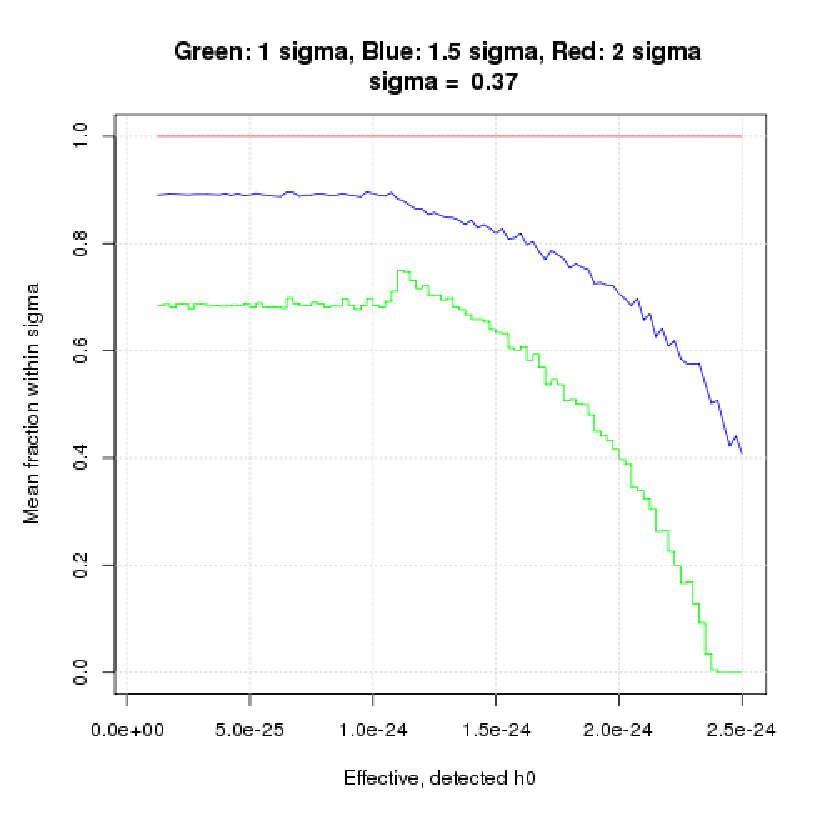
\includegraphics[width=0.3\paperwidth,height=0.2\paperheight]{PlotSigmaDiffVsH0Eff.eps}
\caption{Confidence intervals with final fit. After optimization and constraint to the region with a full bijective mapping between injected and recovered strains (below $1 \times 10^{-24}$), a one-sigma value of 0.37 in the slope was found to give accurate confidence intervals.
}
\end{center}
\end{figure}



The chosen $1.74 \pm 0.37 \sigma$, however, yielded the necessary correction factor.

Finally, we tested all of our calibration factors for h0 with the associated confidence intervals and found the fraction of open data estimated h0, f and asini within their 1 sigma error bars. The results were conservative:

h0: 0.7741935 (77.4\%)
f: 0.7419355 (74.2\%)
asini: 0.6774194 (67.7\%)
Period: 1.00 (100\%) [n.b., we only tested one period, 68023.8259 s]

These error bars were then used without modification for claiming uncertainties on the closed pulsars.


%\end{frame}

\section{Plans for improvement}
%\begin{frame}{Plans for improvement}

\begin{itemize}
\item \emph{Coherently combine multiple interferometer outputs: }\\
Add complex Fourier coefficients (with phase corrections)\\
to create a multi-detector statistic
\item \emph{Elliptical polarization:}\\
search antenna pattern weightings corresponding to\\
elliptical polarization -- better sensitivity
\item \emph{Orbital phase:}\\
Search over initial orbital phase by coherently combining\\
template and doubly Fourier-transformed data
\end{itemize}
%\end{frame}


Other ideas abound. The idea of simulated annealing has arisen in personal communication (e.g., with Maria Alessandra Papa, Sam Finn and others), but it is generally though to address the wrong issues in our high-noise, weak-signal analyses. Also proposed there (and in personal communication with Ethan Obie Romero-Severson) were `hill-climbers' that could explore the parameter space until encountering one of the $X$-pattern arms. Again, due to the low SNR of our expected signals and the availability of computational resources being sufficient, this climbing strategy will probably not be necessary yet (one could imagine it being appropriate for a laptop looking for pulsars in third-generation detector data). It does, however, raise the question of the nature of the $X$-arms.

            How big are the $X$ patterns in the $R$ surface on the modulation depth versus frequency plane?
These $X$-patterns follow the lines $df = f_{\textup{signal}} \pm (f - f_\textup{signal})$, intersecting at $f_\textup{signal}$.

We expect the $X$ pattern to be where the template touches a peak or trough in the time-frequency plane, with an $R$ proportional to the peak in a way that is as the relative power of that bin compared the power in the whole sinusoid. 
Since the template touches only once per period, the ratio would be $T_{\textup{coh}} / P_{\textup{signal}}$. For Scorpius X-1 ($P = 68023.8259$ s), that would lead to ratios of roughly $0.026 \approx 1/38$ for 1800 s SFTs, $0.01 \approx 1/81$ for 840 s SFTs, and $0.0053 \approx 1/189$ for 360 s SFTs.

Yet in practice, as exemplified by pulsar 40 in the Mock Data Challenge, which used 360 s SFTs, the difference between the peak (correct template) $R$-value and the $X$-pattern arms was only a factor of 1/2 to 1/3.
This suggests that the `touch-at-one-point' model is oversimplified, and there is significant overlap still.
There would be a shearing process as $df$ deviates further from the true modulation depth, governed by the frequency bin resolution, $1/T_\textup{coh}$. 
For pulsar 40, $df = 0.046$ Hz, the amplitude of this modulation depth was only about $B = \left(2 \pi \textup{asini} f / P \right) \times \textup{coh} \approx $ 16 bins, with a period of 189 bins.
We could estimate the fractional power in the arms to then be $2 \pi / \cos^{-1} ((B-1) / B)$, or roughly $1/18$ for pulsar 40.
Taking the arccosine of $(B-2)/B$ instead yields roughly $1/12$.
This is closer to the 1/2 to 1/3 ratios observed in the analyses that than 1/189 predicted naively, although a proper study would require a closer look at the generation of TwoSpect \textit{exact templates}.

The deeper problem is that the wrong putative template and the true signal are both stationary are the same point in the time-frequency plane, stationary in the sense that their derivatives match:

\begin{equation}
\frac{df_\textup{true} (t)}{dt} = \frac{df_\textup{template}(t)}{dt} = 0.
\end{equation}

Understanding the $X$ structure more fully could inform future methods for maximum likelihood estimation on the $R$ statistic plane or, more likely, on the pushed-forward $p-value$ plane.
Theoretically, combining information from across the parameter space plane should create a strong signal.
This approach could parallel the deconvolution of point spread functions in optical imaging.
Although the deconvolution or Green's function would be different, this might also enhance the angular resolution when applied to spread on the right ascension, declination plane.
Constructing the deconvolved plane should in principle yield the same information as constructing a likelihood surface.
However, this approach needs to be tested.

An \textit{ansatz} of the point spread function made by summing a given pixel with the appropriate nearby diagonal neighbors was coded as a toy model in Python, with the resulting heatmap indeed being more square and less $X$-shaped near the injection template. However, the signal-to-noise ratio (mean subtracted number of standard deviations at peak) was reduced by a factor of about $7/4$. This suggests more research into an appropriate kernel would be needed for this method to be a success, although in principle the additional information in the $X$ arms should contribute information to a search. 

\section{Summary}
%\begin{frame}{Summary}
%\subsection{General summary for TwoSpect}


\emph{Binary search summary}
\begin{itemize}
\item TwoSpect well-suited to Scorpius X-1 mock data challenges
\item Pursuing real Scorpius X-1 (and J1751-305) searches soon
\item Directed binary searches can be more sensitive with straightforward
changes
\end{itemize}

%\emph{Acknowledgments}


%Thanks to the American Physical Society for hosting this conference,
%as well as the University of Michigan, Evan Goetz for introducing
%TwoSpect, Keith Riles for guidance, and the LIGO Scientific Collaboration
%and National Science Foundation.

%\end{frame}

%\begin{frame}{Bibliography}


\emph{References}


\cite{Chakrabarty2003,GoetzThesis,GoetzTwoSpectMethods2011,PapaloizouPringle1978,Wagoner1984}


%\bibliographystyle{apsrev}
%\bibliography{bibliography}



%\part{Appendix}

%\end{frame}

%\begin{frame}{Scorpius X-1 parameters}
\subsection{Scorpius X-1 parameters}

\begin{itemize}
\item Distance: 9000 light-years (2.8 kpc)
\item Eccentricity: $<3\times10^{-3}$
\item Sky location: $\alpha$=16h19m55.1s, $\delta$=-15d38m24.9s
\item X-ray luminosity: 2.3 $\times10^{31}$W, 60000 $L_{Sol}$
\item First LIGO search: Phys. Rev. D 76 (2007) 082001; gr-qc/0605028
\item Torque-balance (Papaloizou and Pringle 1978) equation (Wagoner 1984),
generally:
\end{itemize}

\[
h_{0}=5\times10^{-27}\left(\frac{300\textup{Hz}}{\nu}\right)^{1/2}\left(\frac{F_{\times}}{10^{-8}\textup{erg cm}^{-2}\textup{s}^{-1}}\right)^{1/2}
\]

\begin{itemize}
\item Sco X-1:
\end{itemize}

\[
h_{0}=3\times10^{-26}\left(\frac{540\textup{Hz}}{f}\right)^{1/2}
\]


%\end{frame}

%\begin{frame}{Polarization addendum}
\subsection{Polarization addendum}


Also note general formula for polarization deriveable from (TwoSpect
results paper)


\[
h(t)=h_{0}F_{\times}(t,\alpha,\delta,\psi)\frac{1+\cos^{2}(\iota)}{2}\cos[\Phi(t)]+
\]



\[
h_{0}F_{+}(t,\alpha,\delta,\psi)\cos(\iota)\sin[\Phi(t)]
\]



Also: fastest known pulsar $f=$716 Hz(?)

%\end{frame}


%\begin{frame}{Coherent interferometer synthesis}
\subsection{Coherent interferometer synthesis}


\textbf{Coherent interferometer synthesis for H1-L1-V1(-?)}


\[
h(f,t)=\Sigma_{j}\left(h_{j}(f,t)+\phi_{j}(f,\alpha,\delta)\right)
\]



\[
\phi_{j}(f,\alpha,\delta)=2\pi fT_{j}(\alpha,\delta)+\phi_{0}
\]



\emph{$h_{j}(f,t)$}: complex $h$ value in SFT for interferometer
$j$, time $t$, frequency $j$


$\phi_{j}(f,\alpha,\delta)$: phase shift for right ascension $\alpha$,
declination $\delta$


(overall phase shift $\phi_{0}$ factors out: 


TwoSpect computes statistic from power)


$T_{j}(\alpha,\delta)$: time-of-flight delay between interferometers 


(projected on vector from $\alpha,\delta$)

%\end{frame}

%\begin{frame}{Circular \& elliptical polarization}
\subsection{Circular \& elliptical polarization}


\textbf{TwoSpect circular polarization assumption generalized}


Current algorithm calculates pixel powers $P$ for SFT $n$, bin $k$:


\[
\tilde{P}_{k}^{n}=\frac{F_{n}^{2}(P_{k}^{n}-<P_{k}>^{n})}{(<P_{k}>^{n})^{2}}\left[\Sigma_{n'}^{N}\frac{F_{n'}^{4}}{(<P_{k}>^{n'})^{2}}\right]^{-1}
\]



\[
F^{2}(t,\alpha,\delta)=F_{\times}^{2}(t,\alpha,\delta)+F_{+}^{2}(t,\alpha,\delta)
\]



$F$: antenna pattern polarization weighting 


as-is, assumes circular polarization


Generalize to elliptical polarization angle $\psi$ with weights $a,b$:


\[
F^{2}(t,\alpha,\delta,\psi)=aF_{\times}^{2}(t,\alpha,\delta,\psi)+bF_{+}^{2}(t,\alpha,\delta,\psi)
\]



Better upper limits; inclination angle $\iota$?

%\end{frame}

%\begin{frame}{Orbital phase \& beyond}
\subsection{Orbital phase \& beyond}


\textbf{Templates for orbital phase in the 2nd Fourier plane}
\begin{itemize}
\item Templates weight 2nd Fourier plane powers
\item Possible: phase in 2nd Fourier bins
\item Benefits: consistency between rows, binary orbital phase?
\item Significant alteration to weighting $\rightarrow$ beyond R statistic
\end{itemize}

\emph{Coherent synthesis, elliptical polarization, orbital phase}


need implementation, validation \& testing


Distributed computing (Einstein@home)?
%\end{frame}

        %---------------------------------

	%The following is an example of using the commands \textit{ref}
	%and \textit{label}. With these commands theorems, chapters,
	%sections and figurres can be labeld with names in the tex file
	%and then refered to by these names in later tex files. In
	%chapter~\ref{intro} we saw section~\ref{sample_section} or
	%theorem~\ref{sample_theorem}.

	%Lastly, here is how to include a figure. First generate an
	%encapsulated postscript file in xfig, adobe illustrator or
	%some other program. The specific commands are found in
	%\textit{chap2.tex}.

        %\begin{figure}[htb]
        %\centerline{ \epsfig{figure=sample.eps, 
        %height =  1.5 in}}
        %\caption{Sample Figure}
        %\label{sample_figure}
        %\end{figure}

